\documentclass[12pt,a4paper]{article}
        \usepackage{graphicx}
        \usepackage{geometry}
        \geometry{margin=2cm}
        \usepackage{helvet}
        \usepackage{xcolor}
        \usepackage{amsmath} % for bmatrix
        \setlength{\parindent}{0pt}  % No indentation globally
        \renewcommand{\familydefault}{\sfdefault}
        \usepackage[german]{babel}% for glqq / grqq

        \begin{document}\begin{center}
                \Huge \textbf{Chlorobenzene} \\[1cm]
                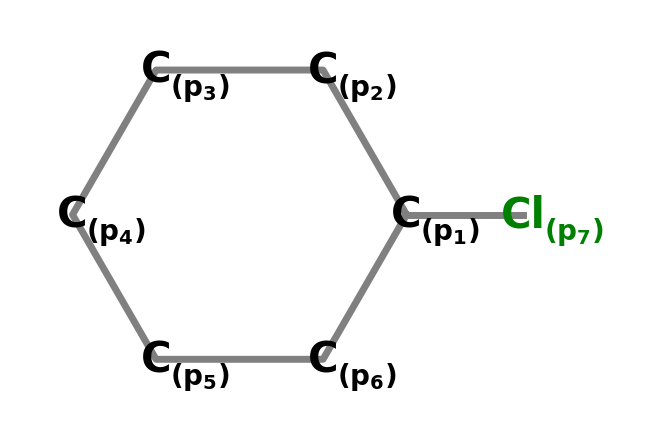
\includegraphics[width=0.5\textwidth]{chlorobenzene} \\[0.5cm]
                \Large Point Group: \textbf{C2v}
            \end{center}\newpage\section*{p orbitals}
Symmetry behavior of the p-orbitals:
$$\mathsf{\Gamma}_{red} = \,7 E\;\oplus{}\,-3 C2\;\oplus{}\,-7 \sigma v(xz)\;\oplus{}\,3 \sigma v(yz)\;$$
$$\mathsf{\Gamma}_{irred} = \,2 A2\;\oplus{}\,5 B2\;$$


\begin{itemize}
\item SALC of B2: \quad $\text{p}_{1}$
\item SALC of A2: \quad $\frac{\sqrt{2} \left(\text{p}_{2} - \text{p}_{6}\right)}{2}$
\item SALC of B2: \quad $\frac{\sqrt{2} \left(\text{p}_{2} + \text{p}_{6}\right)}{2}$
\item SALC of A2: \quad $\frac{\sqrt{2} \left(\text{p}_{3} - \text{p}_{5}\right)}{2}$
\item SALC of B2: \quad $\frac{\sqrt{2} \left(\text{p}_{3} + \text{p}_{5}\right)}{2}$
\item SALC of B2: \quad $\text{p}_{4}$
\item SALC of B2: \quad $\text{p}_{7}$
\end{itemize}
Put together these SALCs form the following Hamilton matrices:
     $$ H_{B2}= \left[\begin{bmatrix}\tilde{\alpha} & \sqrt{2} \tilde{\beta} & 0 & 0 & \tilde{\beta}_{Cl}\\\sqrt{2} \tilde{\beta} & \tilde{\alpha} & \tilde{\beta} & 0 & 0\\0 & \tilde{\beta} & \tilde{\alpha} & \sqrt{2} \tilde{\beta} & 0\\0 & 0 & \sqrt{2} \tilde{\beta} & \tilde{\alpha} & 0\\\tilde{\beta}_{Cl} & 0 & 0 & 0 & \tilde{\alpha}_{Cl}\end{bmatrix}\right]$$ 
     $$ H_{A2}= \left[\begin{bmatrix}\tilde{\alpha} & \tilde{\beta}\\\tilde{\beta} & \tilde{\alpha}\end{bmatrix}\right]$$ 


Solving Hückels secular equations, that follow from these H, leads to:
\begin{itemize}
\item orbital of A2 with energy = 
                                $\tilde{\alpha} + \tilde{\beta}$ \\
( 
$$
\left[\begin{matrix}\frac{\sqrt{2}}{2} & \frac{\sqrt{2}}{2}\end{matrix}\right] * \left[\begin{array}{c}\text{1. SALC in A2} \\ \text{2. SALC in A2}\end{array}\right] = \left[\begin{matrix}\frac{\sqrt{2}}{2} & \frac{\sqrt{2}}{2}\end{matrix}\right] * \left[\begin{matrix}\frac{\sqrt{2} \text{p}_{2}}{2} - \frac{\sqrt{2} \text{p}_{6}}{2}\\\frac{\sqrt{2} \text{p}_{3}}{2} - \frac{\sqrt{2} \text{p}_{5}}{2}\end{matrix}\right] 
 $$ $$ = \frac{\text{p}_{2}}{2} + \frac{\text{p}_{3}}{2} - \frac{\text{p}_{5}}{2} - \frac{\text{p}_{6}}{2} 
 $$ 
 )

\item orbital of A2 with energy = 
                                $\tilde{\alpha} - \tilde{\beta}$ \\
( 
$$
\left[\begin{matrix}- \frac{\sqrt{2}}{2} & \frac{\sqrt{2}}{2}\end{matrix}\right] * \left[\begin{array}{c}\text{1. SALC in A2} \\ \text{2. SALC in A2}\end{array}\right] = \left[\begin{matrix}- \frac{\sqrt{2}}{2} & \frac{\sqrt{2}}{2}\end{matrix}\right] * \left[\begin{matrix}\frac{\sqrt{2} \text{p}_{2}}{2} - \frac{\sqrt{2} \text{p}_{6}}{2}\\\frac{\sqrt{2} \text{p}_{3}}{2} - \frac{\sqrt{2} \text{p}_{5}}{2}\end{matrix}\right] 
 $$ $$ = - \frac{\text{p}_{2}}{2} + \frac{\text{p}_{3}}{2} - \frac{\text{p}_{5}}{2} + \frac{\text{p}_{6}}{2} 
 $$ 
 )

\item orbital of B2 with energy = 
                                $E0(B2)$ \\
( 
$$
\left[\begin{matrix}?_{1} Norm^{2} & ?_{2} Norm^{2} & ?_{3} Norm^{2} & ?_{4} Norm^{2} & ?_{5} Norm^{2}\end{matrix}\right] * \left[\begin{array}{c}\text{1. SALC in B2} \\ \text{2. SALC in B2} \\ \text{3. SALC in B2} \\ \text{4. SALC in B2} \\ \text{5. SALC in B2}\end{array}\right] = \left[\begin{matrix}?_{1} Norm^{2} & ?_{2} Norm^{2} & ?_{3} Norm^{2} & ?_{4} Norm^{2} & ?_{5} Norm^{2}\end{matrix}\right] * \left[\begin{matrix}\text{p}_{1}\\\frac{\sqrt{2} \text{p}_{2}}{2} + \frac{\sqrt{2} \text{p}_{6}}{2}\\\frac{\sqrt{2} \text{p}_{3}}{2} + \frac{\sqrt{2} \text{p}_{5}}{2}\\\text{p}_{4}\\\text{p}_{7}\end{matrix}\right] 
 $$ $$ = ?_{1} Norm^{2} \text{p}_{1} + ?_{2} Norm^{2} \left(\frac{\sqrt{2} \text{p}_{2}}{2} + \frac{\sqrt{2} \text{p}_{6}}{2}\right) + ?_{3} Norm^{2} \left(\frac{\sqrt{2} \text{p}_{3}}{2} + \frac{\sqrt{2} \text{p}_{5}}{2}\right) + ?_{4} Norm^{2} \text{p}_{4} + ?_{5} Norm^{2} \text{p}_{7} 
 $$ 
 )

\item orbital of B2 with energy = 
                                $E1(B2)$ \\
( 
$$
\left[\begin{matrix}?_{1} Norm^{2} & ?_{2} Norm^{2} & ?_{3} Norm^{2} & ?_{4} Norm^{2} & ?_{5} Norm^{2}\end{matrix}\right] * \left[\begin{array}{c}\text{1. SALC in B2} \\ \text{2. SALC in B2} \\ \text{3. SALC in B2} \\ \text{4. SALC in B2} \\ \text{5. SALC in B2}\end{array}\right] = \left[\begin{matrix}?_{1} Norm^{2} & ?_{2} Norm^{2} & ?_{3} Norm^{2} & ?_{4} Norm^{2} & ?_{5} Norm^{2}\end{matrix}\right] * \left[\begin{matrix}\text{p}_{1}\\\frac{\sqrt{2} \text{p}_{2}}{2} + \frac{\sqrt{2} \text{p}_{6}}{2}\\\frac{\sqrt{2} \text{p}_{3}}{2} + \frac{\sqrt{2} \text{p}_{5}}{2}\\\text{p}_{4}\\\text{p}_{7}\end{matrix}\right] 
 $$ $$ = ?_{1} Norm^{2} \text{p}_{1} + ?_{2} Norm^{2} \left(\frac{\sqrt{2} \text{p}_{2}}{2} + \frac{\sqrt{2} \text{p}_{6}}{2}\right) + ?_{3} Norm^{2} \left(\frac{\sqrt{2} \text{p}_{3}}{2} + \frac{\sqrt{2} \text{p}_{5}}{2}\right) + ?_{4} Norm^{2} \text{p}_{4} + ?_{5} Norm^{2} \text{p}_{7} 
 $$ 
 )

\item orbital of B2 with energy = 
                                $E2(B2)$ \\
( 
$$
\left[\begin{matrix}?_{1} Norm^{2} & ?_{2} Norm^{2} & ?_{3} Norm^{2} & ?_{4} Norm^{2} & ?_{5} Norm^{2}\end{matrix}\right] * \left[\begin{array}{c}\text{1. SALC in B2} \\ \text{2. SALC in B2} \\ \text{3. SALC in B2} \\ \text{4. SALC in B2} \\ \text{5. SALC in B2}\end{array}\right] = \left[\begin{matrix}?_{1} Norm^{2} & ?_{2} Norm^{2} & ?_{3} Norm^{2} & ?_{4} Norm^{2} & ?_{5} Norm^{2}\end{matrix}\right] * \left[\begin{matrix}\text{p}_{1}\\\frac{\sqrt{2} \text{p}_{2}}{2} + \frac{\sqrt{2} \text{p}_{6}}{2}\\\frac{\sqrt{2} \text{p}_{3}}{2} + \frac{\sqrt{2} \text{p}_{5}}{2}\\\text{p}_{4}\\\text{p}_{7}\end{matrix}\right] 
 $$ $$ = ?_{1} Norm^{2} \text{p}_{1} + ?_{2} Norm^{2} \left(\frac{\sqrt{2} \text{p}_{2}}{2} + \frac{\sqrt{2} \text{p}_{6}}{2}\right) + ?_{3} Norm^{2} \left(\frac{\sqrt{2} \text{p}_{3}}{2} + \frac{\sqrt{2} \text{p}_{5}}{2}\right) + ?_{4} Norm^{2} \text{p}_{4} + ?_{5} Norm^{2} \text{p}_{7} 
 $$ 
 )

\item orbital of B2 with energy = 
                                $E3(B2)$ \\
( 
$$
\left[\begin{matrix}?_{1} Norm^{2} & ?_{2} Norm^{2} & ?_{3} Norm^{2} & ?_{4} Norm^{2} & ?_{5} Norm^{2}\end{matrix}\right] * \left[\begin{array}{c}\text{1. SALC in B2} \\ \text{2. SALC in B2} \\ \text{3. SALC in B2} \\ \text{4. SALC in B2} \\ \text{5. SALC in B2}\end{array}\right] = \left[\begin{matrix}?_{1} Norm^{2} & ?_{2} Norm^{2} & ?_{3} Norm^{2} & ?_{4} Norm^{2} & ?_{5} Norm^{2}\end{matrix}\right] * \left[\begin{matrix}\text{p}_{1}\\\frac{\sqrt{2} \text{p}_{2}}{2} + \frac{\sqrt{2} \text{p}_{6}}{2}\\\frac{\sqrt{2} \text{p}_{3}}{2} + \frac{\sqrt{2} \text{p}_{5}}{2}\\\text{p}_{4}\\\text{p}_{7}\end{matrix}\right] 
 $$ $$ = ?_{1} Norm^{2} \text{p}_{1} + ?_{2} Norm^{2} \left(\frac{\sqrt{2} \text{p}_{2}}{2} + \frac{\sqrt{2} \text{p}_{6}}{2}\right) + ?_{3} Norm^{2} \left(\frac{\sqrt{2} \text{p}_{3}}{2} + \frac{\sqrt{2} \text{p}_{5}}{2}\right) + ?_{4} Norm^{2} \text{p}_{4} + ?_{5} Norm^{2} \text{p}_{7} 
 $$ 
 )

\item orbital of B2 with energy = 
                                $E4(B2)$ \\
( 
$$
\left[\begin{matrix}?_{1} Norm^{2} & ?_{2} Norm^{2} & ?_{3} Norm^{2} & ?_{4} Norm^{2} & ?_{5} Norm^{2}\end{matrix}\right] * \left[\begin{array}{c}\text{1. SALC in B2} \\ \text{2. SALC in B2} \\ \text{3. SALC in B2} \\ \text{4. SALC in B2} \\ \text{5. SALC in B2}\end{array}\right] = \left[\begin{matrix}?_{1} Norm^{2} & ?_{2} Norm^{2} & ?_{3} Norm^{2} & ?_{4} Norm^{2} & ?_{5} Norm^{2}\end{matrix}\right] * \left[\begin{matrix}\text{p}_{1}\\\frac{\sqrt{2} \text{p}_{2}}{2} + \frac{\sqrt{2} \text{p}_{6}}{2}\\\frac{\sqrt{2} \text{p}_{3}}{2} + \frac{\sqrt{2} \text{p}_{5}}{2}\\\text{p}_{4}\\\text{p}_{7}\end{matrix}\right] 
 $$ $$ = ?_{1} Norm^{2} \text{p}_{1} + ?_{2} Norm^{2} \left(\frac{\sqrt{2} \text{p}_{2}}{2} + \frac{\sqrt{2} \text{p}_{6}}{2}\right) + ?_{3} Norm^{2} \left(\frac{\sqrt{2} \text{p}_{3}}{2} + \frac{\sqrt{2} \text{p}_{5}}{2}\right) + ?_{4} Norm^{2} \text{p}_{4} + ?_{5} Norm^{2} \text{p}_{7} 
 $$ 
 )

\end{itemize}



\newpage \section*{s orbitals}
Symmetry behavior of the s-orbitals:
$$\mathsf{\Gamma}_{red} = \,7 E\;\oplus{}\,3 C2\;\oplus{}\,7 \sigma v(xz)\;\oplus{}\,3 \sigma v(yz)\;$$
$$\mathsf{\Gamma}_{irred} = \,5 A1\;\oplus{}\,2 B1\;$$


\begin{itemize}
\item SALC of A1: \quad $\text{s}_{1}$
\item SALC of A1: \quad $\frac{\sqrt{2} \left(\text{s}_{2} + \text{s}_{6}\right)}{2}$
\item SALC of B1: \quad $\frac{\sqrt{2} \left(\text{s}_{2} - \text{s}_{6}\right)}{2}$
\item SALC of A1: \quad $\frac{\sqrt{2} \left(\text{s}_{3} + \text{s}_{5}\right)}{2}$
\item SALC of B1: \quad $\frac{\sqrt{2} \left(\text{s}_{3} - \text{s}_{5}\right)}{2}$
\item SALC of A1: \quad $\text{s}_{4}$
\item SALC of A1: \quad $\text{s}_{7}$
\end{itemize}
Put together these SALCs form the following Hamilton matrices:
     $$ H_{A1}= \left[\begin{bmatrix}\tilde{\alpha}_{s} & \sqrt{2} \tilde{\beta}_{s} & 0 & 0 & beta_{\text{s}_Cl}\\\sqrt{2} \tilde{\beta}_{s} & \tilde{\alpha}_{s} & \tilde{\beta}_{s} & 0 & 0\\0 & \tilde{\beta}_{s} & \tilde{\alpha}_{s} & \sqrt{2} \tilde{\beta}_{s} & 0\\0 & 0 & \sqrt{2} \tilde{\beta}_{s} & \tilde{\alpha}_{s} & 0\\tilde{\beta}_{\text{s}_Cl} & 0 & 0 & 0 & alpha_{\text{s}_Cl}\end{bmatrix}\right]$$ 
     $$ H_{B1}= \left[\begin{bmatrix}\tilde{\alpha}_{s} & \tilde{\beta}_{s}\\\tilde{\beta}_{s} & \tilde{\alpha}_{s}\end{bmatrix}\right]$$ 


Solving Hückels secular equations, that follow from these H, leads to:
\begin{itemize}
\item orbital of B1 with energy = 
                                $\tilde{\alpha}_{s} + \tilde{\beta}_{s}$ \\
( 
$$
\left[\begin{matrix}\frac{\sqrt{2}}{2} & \frac{\sqrt{2}}{2}\end{matrix}\right] * \left[\begin{array}{c}\text{1. SALC in B1} \\ \text{2. SALC in B1}\end{array}\right] = \left[\begin{matrix}\frac{\sqrt{2}}{2} & \frac{\sqrt{2}}{2}\end{matrix}\right] * \left[\begin{matrix}\frac{\sqrt{2} \text{s}_{2}}{2} - \frac{\sqrt{2} \text{s}_{6}}{2}\\\frac{\sqrt{2} \text{s}_{3}}{2} - \frac{\sqrt{2} \text{s}_{5}}{2}\end{matrix}\right] 
 $$ $$ = \frac{\text{s}_{2}}{2} + \frac{\text{s}_{3}}{2} - \frac{\text{s}_{5}}{2} - \frac{\text{s}_{6}}{2} 
 $$ 
 )

\item orbital of B1 with energy = 
                                $\tilde{\alpha}_{s} - \tilde{\beta}_{s}$ \\
( 
$$
\left[\begin{matrix}- \frac{\sqrt{2}}{2} & \frac{\sqrt{2}}{2}\end{matrix}\right] * \left[\begin{array}{c}\text{1. SALC in B1} \\ \text{2. SALC in B1}\end{array}\right] = \left[\begin{matrix}- \frac{\sqrt{2}}{2} & \frac{\sqrt{2}}{2}\end{matrix}\right] * \left[\begin{matrix}\frac{\sqrt{2} \text{s}_{2}}{2} - \frac{\sqrt{2} \text{s}_{6}}{2}\\\frac{\sqrt{2} \text{s}_{3}}{2} - \frac{\sqrt{2} \text{s}_{5}}{2}\end{matrix}\right] 
 $$ $$ = - \frac{\text{s}_{2}}{2} + \frac{\text{s}_{3}}{2} - \frac{\text{s}_{5}}{2} + \frac{\text{s}_{6}}{2} 
 $$ 
 )

\item orbital of A1 with energy = 
                                $E0(A1)$ \\
( 
$$
\left[\begin{matrix}?_{1} Norm^{2} & ?_{2} Norm^{2} & ?_{3} Norm^{2} & ?_{4} Norm^{2} & ?_{5} Norm^{2}\end{matrix}\right] * \left[\begin{array}{c}\text{1. SALC in A1} \\ \text{2. SALC in A1} \\ \text{3. SALC in A1} \\ \text{4. SALC in A1} \\ \text{5. SALC in A1}\end{array}\right] = \left[\begin{matrix}?_{1} Norm^{2} & ?_{2} Norm^{2} & ?_{3} Norm^{2} & ?_{4} Norm^{2} & ?_{5} Norm^{2}\end{matrix}\right] * \left[\begin{matrix}\text{s}_{1}\\\frac{\sqrt{2} \text{s}_{2}}{2} + \frac{\sqrt{2} \text{s}_{6}}{2}\\\frac{\sqrt{2} \text{s}_{3}}{2} + \frac{\sqrt{2} \text{s}_{5}}{2}\\\text{s}_{4}\\\text{s}_{7}\end{matrix}\right] 
 $$ $$ = ?_{1} Norm^{2} \text{s}_{1} + ?_{2} Norm^{2} \left(\frac{\sqrt{2} \text{s}_{2}}{2} + \frac{\sqrt{2} \text{s}_{6}}{2}\right) + ?_{3} Norm^{2} \left(\frac{\sqrt{2} \text{s}_{3}}{2} + \frac{\sqrt{2} \text{s}_{5}}{2}\right) + ?_{4} Norm^{2} \text{s}_{4} + ?_{5} Norm^{2} \text{s}_{7} 
 $$ 
 )

\item orbital of A1 with energy = 
                                $E1(A1)$ \\
( 
$$
\left[\begin{matrix}?_{1} Norm^{2} & ?_{2} Norm^{2} & ?_{3} Norm^{2} & ?_{4} Norm^{2} & ?_{5} Norm^{2}\end{matrix}\right] * \left[\begin{array}{c}\text{1. SALC in A1} \\ \text{2. SALC in A1} \\ \text{3. SALC in A1} \\ \text{4. SALC in A1} \\ \text{5. SALC in A1}\end{array}\right] = \left[\begin{matrix}?_{1} Norm^{2} & ?_{2} Norm^{2} & ?_{3} Norm^{2} & ?_{4} Norm^{2} & ?_{5} Norm^{2}\end{matrix}\right] * \left[\begin{matrix}\text{s}_{1}\\\frac{\sqrt{2} \text{s}_{2}}{2} + \frac{\sqrt{2} \text{s}_{6}}{2}\\\frac{\sqrt{2} \text{s}_{3}}{2} + \frac{\sqrt{2} \text{s}_{5}}{2}\\\text{s}_{4}\\\text{s}_{7}\end{matrix}\right] 
 $$ $$ = ?_{1} Norm^{2} \text{s}_{1} + ?_{2} Norm^{2} \left(\frac{\sqrt{2} \text{s}_{2}}{2} + \frac{\sqrt{2} \text{s}_{6}}{2}\right) + ?_{3} Norm^{2} \left(\frac{\sqrt{2} \text{s}_{3}}{2} + \frac{\sqrt{2} \text{s}_{5}}{2}\right) + ?_{4} Norm^{2} \text{s}_{4} + ?_{5} Norm^{2} \text{s}_{7} 
 $$ 
 )

\item orbital of A1 with energy = 
                                $E2(A1)$ \\
( 
$$
\left[\begin{matrix}?_{1} Norm^{2} & ?_{2} Norm^{2} & ?_{3} Norm^{2} & ?_{4} Norm^{2} & ?_{5} Norm^{2}\end{matrix}\right] * \left[\begin{array}{c}\text{1. SALC in A1} \\ \text{2. SALC in A1} \\ \text{3. SALC in A1} \\ \text{4. SALC in A1} \\ \text{5. SALC in A1}\end{array}\right] = \left[\begin{matrix}?_{1} Norm^{2} & ?_{2} Norm^{2} & ?_{3} Norm^{2} & ?_{4} Norm^{2} & ?_{5} Norm^{2}\end{matrix}\right] * \left[\begin{matrix}\text{s}_{1}\\\frac{\sqrt{2} \text{s}_{2}}{2} + \frac{\sqrt{2} \text{s}_{6}}{2}\\\frac{\sqrt{2} \text{s}_{3}}{2} + \frac{\sqrt{2} \text{s}_{5}}{2}\\\text{s}_{4}\\\text{s}_{7}\end{matrix}\right] 
 $$ $$ = ?_{1} Norm^{2} \text{s}_{1} + ?_{2} Norm^{2} \left(\frac{\sqrt{2} \text{s}_{2}}{2} + \frac{\sqrt{2} \text{s}_{6}}{2}\right) + ?_{3} Norm^{2} \left(\frac{\sqrt{2} \text{s}_{3}}{2} + \frac{\sqrt{2} \text{s}_{5}}{2}\right) + ?_{4} Norm^{2} \text{s}_{4} + ?_{5} Norm^{2} \text{s}_{7} 
 $$ 
 )

\item orbital of A1 with energy = 
                                $E3(A1)$ \\
( 
$$
\left[\begin{matrix}?_{1} Norm^{2} & ?_{2} Norm^{2} & ?_{3} Norm^{2} & ?_{4} Norm^{2} & ?_{5} Norm^{2}\end{matrix}\right] * \left[\begin{array}{c}\text{1. SALC in A1} \\ \text{2. SALC in A1} \\ \text{3. SALC in A1} \\ \text{4. SALC in A1} \\ \text{5. SALC in A1}\end{array}\right] = \left[\begin{matrix}?_{1} Norm^{2} & ?_{2} Norm^{2} & ?_{3} Norm^{2} & ?_{4} Norm^{2} & ?_{5} Norm^{2}\end{matrix}\right] * \left[\begin{matrix}\text{s}_{1}\\\frac{\sqrt{2} \text{s}_{2}}{2} + \frac{\sqrt{2} \text{s}_{6}}{2}\\\frac{\sqrt{2} \text{s}_{3}}{2} + \frac{\sqrt{2} \text{s}_{5}}{2}\\\text{s}_{4}\\\text{s}_{7}\end{matrix}\right] 
 $$ $$ = ?_{1} Norm^{2} \text{s}_{1} + ?_{2} Norm^{2} \left(\frac{\sqrt{2} \text{s}_{2}}{2} + \frac{\sqrt{2} \text{s}_{6}}{2}\right) + ?_{3} Norm^{2} \left(\frac{\sqrt{2} \text{s}_{3}}{2} + \frac{\sqrt{2} \text{s}_{5}}{2}\right) + ?_{4} Norm^{2} \text{s}_{4} + ?_{5} Norm^{2} \text{s}_{7} 
 $$ 
 )

\item orbital of A1 with energy = 
                                $E4(A1)$ \\
( 
$$
\left[\begin{matrix}?_{1} Norm^{2} & ?_{2} Norm^{2} & ?_{3} Norm^{2} & ?_{4} Norm^{2} & ?_{5} Norm^{2}\end{matrix}\right] * \left[\begin{array}{c}\text{1. SALC in A1} \\ \text{2. SALC in A1} \\ \text{3. SALC in A1} \\ \text{4. SALC in A1} \\ \text{5. SALC in A1}\end{array}\right] = \left[\begin{matrix}?_{1} Norm^{2} & ?_{2} Norm^{2} & ?_{3} Norm^{2} & ?_{4} Norm^{2} & ?_{5} Norm^{2}\end{matrix}\right] * \left[\begin{matrix}\text{s}_{1}\\\frac{\sqrt{2} \text{s}_{2}}{2} + \frac{\sqrt{2} \text{s}_{6}}{2}\\\frac{\sqrt{2} \text{s}_{3}}{2} + \frac{\sqrt{2} \text{s}_{5}}{2}\\\text{s}_{4}\\\text{s}_{7}\end{matrix}\right] 
 $$ $$ = ?_{1} Norm^{2} \text{s}_{1} + ?_{2} Norm^{2} \left(\frac{\sqrt{2} \text{s}_{2}}{2} + \frac{\sqrt{2} \text{s}_{6}}{2}\right) + ?_{3} Norm^{2} \left(\frac{\sqrt{2} \text{s}_{3}}{2} + \frac{\sqrt{2} \text{s}_{5}}{2}\right) + ?_{4} Norm^{2} \text{s}_{4} + ?_{5} Norm^{2} \text{s}_{7} 
 $$ 
 )

\end{itemize}



\newpage \section*{Transitions from p orbitals into s orbitals}\subsection*{State with Occupation [2, 2, 2, 0, 0, 0, 2] (0 unpaired electrons, mult 1.0)}
        \noindent\textbf{Transition from $\psi_{2}$ into $\psi_{\text{s}_{2}}$:}
        \begin{itemize}
            \item $- [2, 2, 2, 0, 0, 0, 2], (0, 0, 0, 0, 0, 0, 0) \rightarrow (2, 1, 2, 0, 0, 0, 2), (0, 1, 0, 0, 0, 0, 0)$
        
            \item $\psi_{2}:$ linear combination = $- \text{p}_{2} + \text{p}_{6}$, \
            energy = $\tilde{\alpha} - \tilde{\beta}$
            
            \item $\eta_{2}:$ linear combination = $- \text{s}_{2} + \text{s}_{6}$, \
            energy = $\tilde{\alpha}_{s} - \tilde{\beta}_{s}$
            
                \item $\Delta$ Energy: $- \tilde{\alpha} + \tilde{\alpha}_{s} + \tilde{\beta} - \tilde{\beta}_{s}$
                \item Energy of State before Excitation: $2 E0(B2) + 2 E4(B2) + 4 \tilde{\alpha}$
                \item Energy of State after Excitation: $2 E0(B2) + 2 E4(B2) + 3 \tilde{\alpha} + \tilde{\alpha}_{s} + \tilde{\beta} - \tilde{\beta}_{s}$
                \item Energy between Average Energies of $\psi$-/$\eta$-orbitals: $\frac{E0(A1)}{7} - \frac{E0(B2)}{7} + \frac{E1(A1)}{7} - \frac{E1(B2)}{7} + \frac{E2(A1)}{7} - \frac{E2(B2)}{7} + \frac{E3(A1)}{7} - \frac{E3(B2)}{7} + \frac{E4(A1)}{7} - \frac{E4(B2)}{7} - \frac{2 \tilde{\alpha}}{7} + \frac{2 \tilde{\alpha}_{s}}{7}$
            
            \item dipole transition moment: $\tilde{\delta}$
        
        \end{itemize}
        

        \noindent\textbf{Transition from $\psi_{3}$ into $\psi_{\text{s}_{3}}$:}
        \begin{itemize}
            \item $- [2, 2, 2, 0, 0, 0, 2], (0, 0, 0, 0, 0, 0, 0) \rightarrow (2, 2, 1, 0, 0, 0, 2), (0, 0, 1, 0, 0, 0, 0)$
        
            \item $\psi_{3}:$ linear combination = $5 ?_{1} Norm^{2} \text{p}_{1}$, \
            energy = $E0(B2)$
            
            \item $\eta_{3}:$ linear combination = $5 ?_{1} Norm^{2} \text{s}_{1}$, \
            energy = $E0(A1)$
            
                \item $\Delta$ Energy: $E0(A1) - E0(B2)$
                \item Energy of State before Excitation: $2 E0(B2) + 2 E4(B2) + 4 \tilde{\alpha}$
                \item Energy of State after Excitation: $E0(A1) + E0(B2) + 2 E4(B2) + 4 \tilde{\alpha}$
                \item Energy between Average Energies of $\psi$-/$\eta$-orbitals: $\frac{E0(A1)}{7} - \frac{E0(B2)}{7} + \frac{E1(A1)}{7} - \frac{E1(B2)}{7} + \frac{E2(A1)}{7} - \frac{E2(B2)}{7} + \frac{E3(A1)}{7} - \frac{E3(B2)}{7} + \frac{E4(A1)}{7} - \frac{E4(B2)}{7} - \frac{2 \tilde{\alpha}}{7} + \frac{2 \tilde{\alpha}_{s}}{7}$
            
            \item dipole transition moment: $?_{1}^{2} Norm^{4} \tilde{\delta} + ?_{2}^{2} Norm^{4} \tilde{\delta} + ?_{3}^{2} Norm^{4} \tilde{\delta} + ?_{4}^{2} Norm^{4} \tilde{\delta} + ?_{5}^{2} Norm^{4} \tilde{\delta}$
        
        \end{itemize}
        
 -  AND 
\subsection*{State with Occupation (2, 1, 1, 1, 1, 0, 2) (4 unpaired electrons, mult 5.0)}
        \noindent\textbf{Transition from $\psi_{2}$ into $\psi_{\text{s}_{2}}$:}
        \begin{itemize}
            \item $- (2, 1, 1, 1, 1, 0, 2), (0, 0, 0, 0, 0, 0, 0) \rightarrow (2, 0, 1, 1, 1, 0, 2), (0, 1, 0, 0, 0, 0, 0)$
        
            \item $\psi_{2}:$ linear combination = $- \text{p}_{2} + \text{p}_{6}$, \
            energy = $\tilde{\alpha} - \tilde{\beta}$
            
            \item $\eta_{2}:$ linear combination = $- \text{s}_{2} + \text{s}_{6}$, \
            energy = $\tilde{\alpha}_{s} - \tilde{\beta}_{s}$
            
                \item $\Delta$ Energy: $- \tilde{\alpha} + \tilde{\alpha}_{s} + \tilde{\beta} - \tilde{\beta}_{s}$
                \item Energy of State before Excitation: $E0(B2) + E1(B2) + E2(B2) + 2 E4(B2) + 3 \tilde{\alpha} + \tilde{\beta}$
                \item Energy of State after Excitation: $E0(B2) + E1(B2) + E2(B2) + 2 E4(B2) + 2 \tilde{\alpha} + \tilde{\alpha}_{s} + 2 \tilde{\beta} - \tilde{\beta}_{s}$
                \item Energy between Average Energies of $\psi$-/$\eta$-orbitals: $\frac{E0(A1)}{7} - \frac{E0(B2)}{7} + \frac{E1(A1)}{7} - \frac{E1(B2)}{7} + \frac{E2(A1)}{7} - \frac{E2(B2)}{7} + \frac{E3(A1)}{7} - \frac{E3(B2)}{7} + \frac{E4(A1)}{7} - \frac{E4(B2)}{7} - \frac{2 \tilde{\alpha}}{7} + \frac{2 \tilde{\alpha}_{s}}{7}$
            
            \item dipole transition moment: $\tilde{\delta}$
        
        \end{itemize}
        

        \noindent\textbf{Transition from $\psi_{3}$ into $\psi_{\text{s}_{3}}$:}
        \begin{itemize}
            \item $- (2, 1, 1, 1, 1, 0, 2), (0, 0, 0, 0, 0, 0, 0) \rightarrow (2, 1, 0, 1, 1, 0, 2), (0, 0, 1, 0, 0, 0, 0)$
        
            \item $\psi_{3}:$ linear combination = $5 ?_{1} Norm^{2} \text{p}_{1}$, \
            energy = $E0(B2)$
            
            \item $\eta_{3}:$ linear combination = $5 ?_{1} Norm^{2} \text{s}_{1}$, \
            energy = $E0(A1)$
            
                \item $\Delta$ Energy: $E0(A1) - E0(B2)$
                \item Energy of State before Excitation: $E0(B2) + E1(B2) + E2(B2) + 2 E4(B2) + 3 \tilde{\alpha} + \tilde{\beta}$
                \item Energy of State after Excitation: $E0(A1) + E1(B2) + E2(B2) + 2 E4(B2) + 3 \tilde{\alpha} + \tilde{\beta}$
                \item Energy between Average Energies of $\psi$-/$\eta$-orbitals: $\frac{E0(A1)}{7} - \frac{E0(B2)}{7} + \frac{E1(A1)}{7} - \frac{E1(B2)}{7} + \frac{E2(A1)}{7} - \frac{E2(B2)}{7} + \frac{E3(A1)}{7} - \frac{E3(B2)}{7} + \frac{E4(A1)}{7} - \frac{E4(B2)}{7} - \frac{2 \tilde{\alpha}}{7} + \frac{2 \tilde{\alpha}_{s}}{7}$
            
            \item dipole transition moment: $?_{1}^{2} Norm^{4} \tilde{\delta} + ?_{2}^{2} Norm^{4} \tilde{\delta} + ?_{3}^{2} Norm^{4} \tilde{\delta} + ?_{4}^{2} Norm^{4} \tilde{\delta} + ?_{5}^{2} Norm^{4} \tilde{\delta}$
        
        \end{itemize}
        
 -  AND 

        \noindent\textbf{Transition from $\psi_{4}$ into $\psi_{\text{s}_{4}}$:}
        \begin{itemize}
            \item $- (2, 1, 1, 1, 1, 0, 2), (0, 0, 0, 0, 0, 0, 0) \rightarrow (2, 1, 1, 0, 1, 0, 2), (0, 0, 0, 1, 0, 0, 0)$
        
            \item $\psi_{4}:$ linear combination = $5 ?_{1} Norm^{2} \text{p}_{1}$, \
            energy = $E1(B2)$
            
            \item $\eta_{4}:$ linear combination = $5 ?_{1} Norm^{2} \text{s}_{1}$, \
            energy = $E1(A1)$
            
                \item $\Delta$ Energy: $E1(A1) - E1(B2)$
                \item Energy of State before Excitation: $E0(B2) + E1(B2) + E2(B2) + 2 E4(B2) + 3 \tilde{\alpha} + \tilde{\beta}$
                \item Energy of State after Excitation: $E0(B2) + E1(A1) + E2(B2) + 2 E4(B2) + 3 \tilde{\alpha} + \tilde{\beta}$
                \item Energy between Average Energies of $\psi$-/$\eta$-orbitals: $\frac{E0(A1)}{7} - \frac{E0(B2)}{7} + \frac{E1(A1)}{7} - \frac{E1(B2)}{7} + \frac{E2(A1)}{7} - \frac{E2(B2)}{7} + \frac{E3(A1)}{7} - \frac{E3(B2)}{7} + \frac{E4(A1)}{7} - \frac{E4(B2)}{7} - \frac{2 \tilde{\alpha}}{7} + \frac{2 \tilde{\alpha}_{s}}{7}$
            
            \item dipole transition moment: $?_{1}^{2} Norm^{4} \tilde{\delta} + ?_{2}^{2} Norm^{4} \tilde{\delta} + ?_{3}^{2} Norm^{4} \tilde{\delta} + ?_{4}^{2} Norm^{4} \tilde{\delta} + ?_{5}^{2} Norm^{4} \tilde{\delta}$
        
        \end{itemize}
        
 -  AND 

        \noindent\textbf{Transition from $\psi_{5}$ into $\psi_{\text{s}_{5}}$:}
        \begin{itemize}
            \item $- (2, 1, 1, 1, 1, 0, 2), (0, 0, 0, 0, 0, 0, 0) \rightarrow (2, 1, 1, 1, 0, 0, 2), (0, 0, 0, 0, 1, 0, 0)$
        
            \item $\psi_{5}:$ linear combination = $5 ?_{1} Norm^{2} \text{p}_{1}$, \
            energy = $E2(B2)$
            
            \item $\eta_{5}:$ linear combination = $5 ?_{1} Norm^{2} \text{s}_{1}$, \
            energy = $E2(A1)$
            
                \item $\Delta$ Energy: $E2(A1) - E2(B2)$
                \item Energy of State before Excitation: $E0(B2) + E1(B2) + E2(B2) + 2 E4(B2) + 3 \tilde{\alpha} + \tilde{\beta}$
                \item Energy of State after Excitation: $E0(B2) + E1(B2) + E2(A1) + 2 E4(B2) + 3 \tilde{\alpha} + \tilde{\beta}$
                \item Energy between Average Energies of $\psi$-/$\eta$-orbitals: $\frac{E0(A1)}{7} - \frac{E0(B2)}{7} + \frac{E1(A1)}{7} - \frac{E1(B2)}{7} + \frac{E2(A1)}{7} - \frac{E2(B2)}{7} + \frac{E3(A1)}{7} - \frac{E3(B2)}{7} + \frac{E4(A1)}{7} - \frac{E4(B2)}{7} - \frac{2 \tilde{\alpha}}{7} + \frac{2 \tilde{\alpha}_{s}}{7}$
            
            \item dipole transition moment: $?_{1}^{2} Norm^{4} \tilde{\delta} + ?_{2}^{2} Norm^{4} \tilde{\delta} + ?_{3}^{2} Norm^{4} \tilde{\delta} + ?_{4}^{2} Norm^{4} \tilde{\delta} + ?_{5}^{2} Norm^{4} \tilde{\delta}$
        
        \end{itemize}
        
 -  AND 
\subsection*{State with Occupation (2, 1, 2, 0, 1, 0, 2) (2 unpaired electrons, mult 3.0)}
        \noindent\textbf{Transition from $\psi_{2}$ into $\psi_{\text{s}_{2}}$:}
        \begin{itemize}
            \item $- (2, 1, 2, 0, 1, 0, 2), (0, 0, 0, 0, 0, 0, 0) \rightarrow (2, 0, 2, 0, 1, 0, 2), (0, 1, 0, 0, 0, 0, 0)$
        
            \item $\psi_{2}:$ linear combination = $- \text{p}_{2} + \text{p}_{6}$, \
            energy = $\tilde{\alpha} - \tilde{\beta}$
            
            \item $\eta_{2}:$ linear combination = $- \text{s}_{2} + \text{s}_{6}$, \
            energy = $\tilde{\alpha}_{s} - \tilde{\beta}_{s}$
            
                \item $\Delta$ Energy: $- \tilde{\alpha} + \tilde{\alpha}_{s} + \tilde{\beta} - \tilde{\beta}_{s}$
                \item Energy of State before Excitation: $2 E0(B2) + E2(B2) + 2 E4(B2) + 3 \tilde{\alpha} + \tilde{\beta}$
                \item Energy of State after Excitation: $2 E0(B2) + E2(B2) + 2 E4(B2) + 2 \tilde{\alpha} + \tilde{\alpha}_{s} + 2 \tilde{\beta} - \tilde{\beta}_{s}$
                \item Energy between Average Energies of $\psi$-/$\eta$-orbitals: $\frac{E0(A1)}{7} - \frac{E0(B2)}{7} + \frac{E1(A1)}{7} - \frac{E1(B2)}{7} + \frac{E2(A1)}{7} - \frac{E2(B2)}{7} + \frac{E3(A1)}{7} - \frac{E3(B2)}{7} + \frac{E4(A1)}{7} - \frac{E4(B2)}{7} - \frac{2 \tilde{\alpha}}{7} + \frac{2 \tilde{\alpha}_{s}}{7}$
            
            \item dipole transition moment: $\tilde{\delta}$
        
        \end{itemize}
        

        \noindent\textbf{Transition from $\psi_{3}$ into $\psi_{\text{s}_{3}}$:}
        \begin{itemize}
            \item $- (2, 1, 2, 0, 1, 0, 2), (0, 0, 0, 0, 0, 0, 0) \rightarrow (2, 1, 1, 0, 1, 0, 2), (0, 0, 1, 0, 0, 0, 0)$
        
            \item $\psi_{3}:$ linear combination = $5 ?_{1} Norm^{2} \text{p}_{1}$, \
            energy = $E0(B2)$
            
            \item $\eta_{3}:$ linear combination = $5 ?_{1} Norm^{2} \text{s}_{1}$, \
            energy = $E0(A1)$
            
                \item $\Delta$ Energy: $E0(A1) - E0(B2)$
                \item Energy of State before Excitation: $2 E0(B2) + E2(B2) + 2 E4(B2) + 3 \tilde{\alpha} + \tilde{\beta}$
                \item Energy of State after Excitation: $E0(A1) + E0(B2) + E2(B2) + 2 E4(B2) + 3 \tilde{\alpha} + \tilde{\beta}$
                \item Energy between Average Energies of $\psi$-/$\eta$-orbitals: $\frac{E0(A1)}{7} - \frac{E0(B2)}{7} + \frac{E1(A1)}{7} - \frac{E1(B2)}{7} + \frac{E2(A1)}{7} - \frac{E2(B2)}{7} + \frac{E3(A1)}{7} - \frac{E3(B2)}{7} + \frac{E4(A1)}{7} - \frac{E4(B2)}{7} - \frac{2 \tilde{\alpha}}{7} + \frac{2 \tilde{\alpha}_{s}}{7}$
            
            \item dipole transition moment: $?_{1}^{2} Norm^{4} \tilde{\delta} + ?_{2}^{2} Norm^{4} \tilde{\delta} + ?_{3}^{2} Norm^{4} \tilde{\delta} + ?_{4}^{2} Norm^{4} \tilde{\delta} + ?_{5}^{2} Norm^{4} \tilde{\delta}$
        
        \end{itemize}
        
 -  AND 

        \noindent\textbf{Transition from $\psi_{5}$ into $\psi_{\text{s}_{5}}$:}
        \begin{itemize}
            \item $- (2, 1, 2, 0, 1, 0, 2), (0, 0, 0, 0, 0, 0, 0) \rightarrow (2, 1, 2, 0, 0, 0, 2), (0, 0, 0, 0, 1, 0, 0)$
        
            \item $\psi_{5}:$ linear combination = $5 ?_{1} Norm^{2} \text{p}_{1}$, \
            energy = $E2(B2)$
            
            \item $\eta_{5}:$ linear combination = $5 ?_{1} Norm^{2} \text{s}_{1}$, \
            energy = $E2(A1)$
            
                \item $\Delta$ Energy: $E2(A1) - E2(B2)$
                \item Energy of State before Excitation: $2 E0(B2) + E2(B2) + 2 E4(B2) + 3 \tilde{\alpha} + \tilde{\beta}$
                \item Energy of State after Excitation: $2 E0(B2) + E2(A1) + 2 E4(B2) + 3 \tilde{\alpha} + \tilde{\beta}$
                \item Energy between Average Energies of $\psi$-/$\eta$-orbitals: $\frac{E0(A1)}{7} - \frac{E0(B2)}{7} + \frac{E1(A1)}{7} - \frac{E1(B2)}{7} + \frac{E2(A1)}{7} - \frac{E2(B2)}{7} + \frac{E3(A1)}{7} - \frac{E3(B2)}{7} + \frac{E4(A1)}{7} - \frac{E4(B2)}{7} - \frac{2 \tilde{\alpha}}{7} + \frac{2 \tilde{\alpha}_{s}}{7}$
            
            \item dipole transition moment: $?_{1}^{2} Norm^{4} \tilde{\delta} + ?_{2}^{2} Norm^{4} \tilde{\delta} + ?_{3}^{2} Norm^{4} \tilde{\delta} + ?_{4}^{2} Norm^{4} \tilde{\delta} + ?_{5}^{2} Norm^{4} \tilde{\delta}$
        
        \end{itemize}
        
 -  AND 
\subsection*{State with Occupation (2, 1, 2, 1, 0, 0, 2) (2 unpaired electrons, mult 3.0)}
        \noindent\textbf{Transition from $\psi_{2}$ into $\psi_{\text{s}_{2}}$:}
        \begin{itemize}
            \item $- (2, 1, 2, 1, 0, 0, 2), (0, 0, 0, 0, 0, 0, 0) \rightarrow (2, 0, 2, 1, 0, 0, 2), (0, 1, 0, 0, 0, 0, 0)$
        
            \item $\psi_{2}:$ linear combination = $- \text{p}_{2} + \text{p}_{6}$, \
            energy = $\tilde{\alpha} - \tilde{\beta}$
            
            \item $\eta_{2}:$ linear combination = $- \text{s}_{2} + \text{s}_{6}$, \
            energy = $\tilde{\alpha}_{s} - \tilde{\beta}_{s}$
            
                \item $\Delta$ Energy: $- \tilde{\alpha} + \tilde{\alpha}_{s} + \tilde{\beta} - \tilde{\beta}_{s}$
                \item Energy of State before Excitation: $2 E0(B2) + E1(B2) + 2 E4(B2) + 3 \tilde{\alpha} + \tilde{\beta}$
                \item Energy of State after Excitation: $2 E0(B2) + E1(B2) + 2 E4(B2) + 2 \tilde{\alpha} + \tilde{\alpha}_{s} + 2 \tilde{\beta} - \tilde{\beta}_{s}$
                \item Energy between Average Energies of $\psi$-/$\eta$-orbitals: $\frac{E0(A1)}{7} - \frac{E0(B2)}{7} + \frac{E1(A1)}{7} - \frac{E1(B2)}{7} + \frac{E2(A1)}{7} - \frac{E2(B2)}{7} + \frac{E3(A1)}{7} - \frac{E3(B2)}{7} + \frac{E4(A1)}{7} - \frac{E4(B2)}{7} - \frac{2 \tilde{\alpha}}{7} + \frac{2 \tilde{\alpha}_{s}}{7}$
            
            \item dipole transition moment: $\tilde{\delta}$
        
        \end{itemize}
        

        \noindent\textbf{Transition from $\psi_{3}$ into $\psi_{\text{s}_{3}}$:}
        \begin{itemize}
            \item $- (2, 1, 2, 1, 0, 0, 2), (0, 0, 0, 0, 0, 0, 0) \rightarrow (2, 1, 1, 1, 0, 0, 2), (0, 0, 1, 0, 0, 0, 0)$
        
            \item $\psi_{3}:$ linear combination = $5 ?_{1} Norm^{2} \text{p}_{1}$, \
            energy = $E0(B2)$
            
            \item $\eta_{3}:$ linear combination = $5 ?_{1} Norm^{2} \text{s}_{1}$, \
            energy = $E0(A1)$
            
                \item $\Delta$ Energy: $E0(A1) - E0(B2)$
                \item Energy of State before Excitation: $2 E0(B2) + E1(B2) + 2 E4(B2) + 3 \tilde{\alpha} + \tilde{\beta}$
                \item Energy of State after Excitation: $E0(A1) + E0(B2) + E1(B2) + 2 E4(B2) + 3 \tilde{\alpha} + \tilde{\beta}$
                \item Energy between Average Energies of $\psi$-/$\eta$-orbitals: $\frac{E0(A1)}{7} - \frac{E0(B2)}{7} + \frac{E1(A1)}{7} - \frac{E1(B2)}{7} + \frac{E2(A1)}{7} - \frac{E2(B2)}{7} + \frac{E3(A1)}{7} - \frac{E3(B2)}{7} + \frac{E4(A1)}{7} - \frac{E4(B2)}{7} - \frac{2 \tilde{\alpha}}{7} + \frac{2 \tilde{\alpha}_{s}}{7}$
            
            \item dipole transition moment: $?_{1}^{2} Norm^{4} \tilde{\delta} + ?_{2}^{2} Norm^{4} \tilde{\delta} + ?_{3}^{2} Norm^{4} \tilde{\delta} + ?_{4}^{2} Norm^{4} \tilde{\delta} + ?_{5}^{2} Norm^{4} \tilde{\delta}$
        
        \end{itemize}
        
 -  AND 

        \noindent\textbf{Transition from $\psi_{4}$ into $\psi_{\text{s}_{4}}$:}
        \begin{itemize}
            \item $- (2, 1, 2, 1, 0, 0, 2), (0, 0, 0, 0, 0, 0, 0) \rightarrow (2, 1, 2, 0, 0, 0, 2), (0, 0, 0, 1, 0, 0, 0)$
        
            \item $\psi_{4}:$ linear combination = $5 ?_{1} Norm^{2} \text{p}_{1}$, \
            energy = $E1(B2)$
            
            \item $\eta_{4}:$ linear combination = $5 ?_{1} Norm^{2} \text{s}_{1}$, \
            energy = $E1(A1)$
            
                \item $\Delta$ Energy: $E1(A1) - E1(B2)$
                \item Energy of State before Excitation: $2 E0(B2) + E1(B2) + 2 E4(B2) + 3 \tilde{\alpha} + \tilde{\beta}$
                \item Energy of State after Excitation: $2 E0(B2) + E1(A1) + 2 E4(B2) + 3 \tilde{\alpha} + \tilde{\beta}$
                \item Energy between Average Energies of $\psi$-/$\eta$-orbitals: $\frac{E0(A1)}{7} - \frac{E0(B2)}{7} + \frac{E1(A1)}{7} - \frac{E1(B2)}{7} + \frac{E2(A1)}{7} - \frac{E2(B2)}{7} + \frac{E3(A1)}{7} - \frac{E3(B2)}{7} + \frac{E4(A1)}{7} - \frac{E4(B2)}{7} - \frac{2 \tilde{\alpha}}{7} + \frac{2 \tilde{\alpha}_{s}}{7}$
            
            \item dipole transition moment: $?_{1}^{2} Norm^{4} \tilde{\delta} + ?_{2}^{2} Norm^{4} \tilde{\delta} + ?_{3}^{2} Norm^{4} \tilde{\delta} + ?_{4}^{2} Norm^{4} \tilde{\delta} + ?_{5}^{2} Norm^{4} \tilde{\delta}$
        
        \end{itemize}
        
 -  AND 
\subsection*{State with Occupation (2, 2, 1, 0, 1, 0, 2) (2 unpaired electrons, mult 3.0)}
        \noindent\textbf{Transition from $\psi_{2}$ into $\psi_{\text{s}_{2}}$:}
        \begin{itemize}
            \item $- (2, 2, 1, 0, 1, 0, 2), (0, 0, 0, 0, 0, 0, 0) \rightarrow (2, 1, 1, 0, 1, 0, 2), (0, 1, 0, 0, 0, 0, 0)$
        
            \item $\psi_{2}:$ linear combination = $- \text{p}_{2} + \text{p}_{6}$, \
            energy = $\tilde{\alpha} - \tilde{\beta}$
            
            \item $\eta_{2}:$ linear combination = $- \text{s}_{2} + \text{s}_{6}$, \
            energy = $\tilde{\alpha}_{s} - \tilde{\beta}_{s}$
            
                \item $\Delta$ Energy: $- \tilde{\alpha} + \tilde{\alpha}_{s} + \tilde{\beta} - \tilde{\beta}_{s}$
                \item Energy of State before Excitation: $E0(B2) + E2(B2) + 2 E4(B2) + 4 \tilde{\alpha}$
                \item Energy of State after Excitation: $E0(B2) + E2(B2) + 2 E4(B2) + 3 \tilde{\alpha} + \tilde{\alpha}_{s} + \tilde{\beta} - \tilde{\beta}_{s}$
                \item Energy between Average Energies of $\psi$-/$\eta$-orbitals: $\frac{E0(A1)}{7} - \frac{E0(B2)}{7} + \frac{E1(A1)}{7} - \frac{E1(B2)}{7} + \frac{E2(A1)}{7} - \frac{E2(B2)}{7} + \frac{E3(A1)}{7} - \frac{E3(B2)}{7} + \frac{E4(A1)}{7} - \frac{E4(B2)}{7} - \frac{2 \tilde{\alpha}}{7} + \frac{2 \tilde{\alpha}_{s}}{7}$
            
            \item dipole transition moment: $\tilde{\delta}$
        
        \end{itemize}
        

        \noindent\textbf{Transition from $\psi_{3}$ into $\psi_{\text{s}_{3}}$:}
        \begin{itemize}
            \item $- (2, 2, 1, 0, 1, 0, 2), (0, 0, 0, 0, 0, 0, 0) \rightarrow (2, 2, 0, 0, 1, 0, 2), (0, 0, 1, 0, 0, 0, 0)$
        
            \item $\psi_{3}:$ linear combination = $5 ?_{1} Norm^{2} \text{p}_{1}$, \
            energy = $E0(B2)$
            
            \item $\eta_{3}:$ linear combination = $5 ?_{1} Norm^{2} \text{s}_{1}$, \
            energy = $E0(A1)$
            
                \item $\Delta$ Energy: $E0(A1) - E0(B2)$
                \item Energy of State before Excitation: $E0(B2) + E2(B2) + 2 E4(B2) + 4 \tilde{\alpha}$
                \item Energy of State after Excitation: $E0(A1) + E2(B2) + 2 E4(B2) + 4 \tilde{\alpha}$
                \item Energy between Average Energies of $\psi$-/$\eta$-orbitals: $\frac{E0(A1)}{7} - \frac{E0(B2)}{7} + \frac{E1(A1)}{7} - \frac{E1(B2)}{7} + \frac{E2(A1)}{7} - \frac{E2(B2)}{7} + \frac{E3(A1)}{7} - \frac{E3(B2)}{7} + \frac{E4(A1)}{7} - \frac{E4(B2)}{7} - \frac{2 \tilde{\alpha}}{7} + \frac{2 \tilde{\alpha}_{s}}{7}$
            
            \item dipole transition moment: $?_{1}^{2} Norm^{4} \tilde{\delta} + ?_{2}^{2} Norm^{4} \tilde{\delta} + ?_{3}^{2} Norm^{4} \tilde{\delta} + ?_{4}^{2} Norm^{4} \tilde{\delta} + ?_{5}^{2} Norm^{4} \tilde{\delta}$
        
        \end{itemize}
        
 -  AND 

        \noindent\textbf{Transition from $\psi_{5}$ into $\psi_{\text{s}_{5}}$:}
        \begin{itemize}
            \item $- (2, 2, 1, 0, 1, 0, 2), (0, 0, 0, 0, 0, 0, 0) \rightarrow (2, 2, 1, 0, 0, 0, 2), (0, 0, 0, 0, 1, 0, 0)$
        
            \item $\psi_{5}:$ linear combination = $5 ?_{1} Norm^{2} \text{p}_{1}$, \
            energy = $E2(B2)$
            
            \item $\eta_{5}:$ linear combination = $5 ?_{1} Norm^{2} \text{s}_{1}$, \
            energy = $E2(A1)$
            
                \item $\Delta$ Energy: $E2(A1) - E2(B2)$
                \item Energy of State before Excitation: $E0(B2) + E2(B2) + 2 E4(B2) + 4 \tilde{\alpha}$
                \item Energy of State after Excitation: $E0(B2) + E2(A1) + 2 E4(B2) + 4 \tilde{\alpha}$
                \item Energy between Average Energies of $\psi$-/$\eta$-orbitals: $\frac{E0(A1)}{7} - \frac{E0(B2)}{7} + \frac{E1(A1)}{7} - \frac{E1(B2)}{7} + \frac{E2(A1)}{7} - \frac{E2(B2)}{7} + \frac{E3(A1)}{7} - \frac{E3(B2)}{7} + \frac{E4(A1)}{7} - \frac{E4(B2)}{7} - \frac{2 \tilde{\alpha}}{7} + \frac{2 \tilde{\alpha}_{s}}{7}$
            
            \item dipole transition moment: $?_{1}^{2} Norm^{4} \tilde{\delta} + ?_{2}^{2} Norm^{4} \tilde{\delta} + ?_{3}^{2} Norm^{4} \tilde{\delta} + ?_{4}^{2} Norm^{4} \tilde{\delta} + ?_{5}^{2} Norm^{4} \tilde{\delta}$
        
        \end{itemize}
        
 -  AND 
\subsection*{State with Occupation (2, 2, 1, 1, 0, 0, 2) (2 unpaired electrons, mult 3.0)}
        \noindent\textbf{Transition from $\psi_{2}$ into $\psi_{\text{s}_{2}}$:}
        \begin{itemize}
            \item $- (2, 2, 1, 1, 0, 0, 2), (0, 0, 0, 0, 0, 0, 0) \rightarrow (2, 1, 1, 1, 0, 0, 2), (0, 1, 0, 0, 0, 0, 0)$
        
            \item $\psi_{2}:$ linear combination = $- \text{p}_{2} + \text{p}_{6}$, \
            energy = $\tilde{\alpha} - \tilde{\beta}$
            
            \item $\eta_{2}:$ linear combination = $- \text{s}_{2} + \text{s}_{6}$, \
            energy = $\tilde{\alpha}_{s} - \tilde{\beta}_{s}$
            
                \item $\Delta$ Energy: $- \tilde{\alpha} + \tilde{\alpha}_{s} + \tilde{\beta} - \tilde{\beta}_{s}$
                \item Energy of State before Excitation: $E0(B2) + E1(B2) + 2 E4(B2) + 4 \tilde{\alpha}$
                \item Energy of State after Excitation: $E0(B2) + E1(B2) + 2 E4(B2) + 3 \tilde{\alpha} + \tilde{\alpha}_{s} + \tilde{\beta} - \tilde{\beta}_{s}$
                \item Energy between Average Energies of $\psi$-/$\eta$-orbitals: $\frac{E0(A1)}{7} - \frac{E0(B2)}{7} + \frac{E1(A1)}{7} - \frac{E1(B2)}{7} + \frac{E2(A1)}{7} - \frac{E2(B2)}{7} + \frac{E3(A1)}{7} - \frac{E3(B2)}{7} + \frac{E4(A1)}{7} - \frac{E4(B2)}{7} - \frac{2 \tilde{\alpha}}{7} + \frac{2 \tilde{\alpha}_{s}}{7}$
            
            \item dipole transition moment: $\tilde{\delta}$
        
        \end{itemize}
        

        \noindent\textbf{Transition from $\psi_{3}$ into $\psi_{\text{s}_{3}}$:}
        \begin{itemize}
            \item $- (2, 2, 1, 1, 0, 0, 2), (0, 0, 0, 0, 0, 0, 0) \rightarrow (2, 2, 0, 1, 0, 0, 2), (0, 0, 1, 0, 0, 0, 0)$
        
            \item $\psi_{3}:$ linear combination = $5 ?_{1} Norm^{2} \text{p}_{1}$, \
            energy = $E0(B2)$
            
            \item $\eta_{3}:$ linear combination = $5 ?_{1} Norm^{2} \text{s}_{1}$, \
            energy = $E0(A1)$
            
                \item $\Delta$ Energy: $E0(A1) - E0(B2)$
                \item Energy of State before Excitation: $E0(B2) + E1(B2) + 2 E4(B2) + 4 \tilde{\alpha}$
                \item Energy of State after Excitation: $E0(A1) + E1(B2) + 2 E4(B2) + 4 \tilde{\alpha}$
                \item Energy between Average Energies of $\psi$-/$\eta$-orbitals: $\frac{E0(A1)}{7} - \frac{E0(B2)}{7} + \frac{E1(A1)}{7} - \frac{E1(B2)}{7} + \frac{E2(A1)}{7} - \frac{E2(B2)}{7} + \frac{E3(A1)}{7} - \frac{E3(B2)}{7} + \frac{E4(A1)}{7} - \frac{E4(B2)}{7} - \frac{2 \tilde{\alpha}}{7} + \frac{2 \tilde{\alpha}_{s}}{7}$
            
            \item dipole transition moment: $?_{1}^{2} Norm^{4} \tilde{\delta} + ?_{2}^{2} Norm^{4} \tilde{\delta} + ?_{3}^{2} Norm^{4} \tilde{\delta} + ?_{4}^{2} Norm^{4} \tilde{\delta} + ?_{5}^{2} Norm^{4} \tilde{\delta}$
        
        \end{itemize}
        
 -  AND 

        \noindent\textbf{Transition from $\psi_{4}$ into $\psi_{\text{s}_{4}}$:}
        \begin{itemize}
            \item $- (2, 2, 1, 1, 0, 0, 2), (0, 0, 0, 0, 0, 0, 0) \rightarrow (2, 2, 1, 0, 0, 0, 2), (0, 0, 0, 1, 0, 0, 0)$
        
            \item $\psi_{4}:$ linear combination = $5 ?_{1} Norm^{2} \text{p}_{1}$, \
            energy = $E1(B2)$
            
            \item $\eta_{4}:$ linear combination = $5 ?_{1} Norm^{2} \text{s}_{1}$, \
            energy = $E1(A1)$
            
                \item $\Delta$ Energy: $E1(A1) - E1(B2)$
                \item Energy of State before Excitation: $E0(B2) + E1(B2) + 2 E4(B2) + 4 \tilde{\alpha}$
                \item Energy of State after Excitation: $E0(B2) + E1(A1) + 2 E4(B2) + 4 \tilde{\alpha}$
                \item Energy between Average Energies of $\psi$-/$\eta$-orbitals: $\frac{E0(A1)}{7} - \frac{E0(B2)}{7} + \frac{E1(A1)}{7} - \frac{E1(B2)}{7} + \frac{E2(A1)}{7} - \frac{E2(B2)}{7} + \frac{E3(A1)}{7} - \frac{E3(B2)}{7} + \frac{E4(A1)}{7} - \frac{E4(B2)}{7} - \frac{2 \tilde{\alpha}}{7} + \frac{2 \tilde{\alpha}_{s}}{7}$
            
            \item dipole transition moment: $?_{1}^{2} Norm^{4} \tilde{\delta} + ?_{2}^{2} Norm^{4} \tilde{\delta} + ?_{3}^{2} Norm^{4} \tilde{\delta} + ?_{4}^{2} Norm^{4} \tilde{\delta} + ?_{5}^{2} Norm^{4} \tilde{\delta}$
        
        \end{itemize}
        
 -  AND 
\newpage \section*{Dispersion energies following from the transitions}

\begin{enumerate}
 \item State: A = [2, 2, 2, 0, 0, 0, 2] $\leftrightarrow$ B = (2, 1, 1, 1, 1, 0, 2) 
$$E_{dispersion} =\frac{8 \tilde{\delta}^{4}}{r^{6} \left(- 2 \tilde{\alpha} + 2 \tilde{\alpha}_{s} + 2 \tilde{\beta} - 2 \tilde{\beta}_{s}\right)} + \frac{8 \tilde{\delta}^{2} \left(?_{1}^{2} Norm^{4} \tilde{\delta} + ?_{2}^{2} Norm^{4} \tilde{\delta} + ?_{3}^{2} Norm^{4} \tilde{\delta} + ?_{4}^{2} Norm^{4} \tilde{\delta} + ?_{5}^{2} Norm^{4} \tilde{\delta}\right)^{2}}{r^{6} \left(E2(A1) - E2(B2) - \tilde{\alpha} + \tilde{\alpha}_{s} + \tilde{\beta} - \tilde{\beta}_{s}\right)} + \frac{8 \tilde{\delta}^{2} \left(?_{1}^{2} Norm^{4} \tilde{\delta} + ?_{2}^{2} Norm^{4} \tilde{\delta} + ?_{3}^{2} Norm^{4} \tilde{\delta} + ?_{4}^{2} Norm^{4} \tilde{\delta} + ?_{5}^{2} Norm^{4} \tilde{\delta}\right)^{2}}{r^{6} \left(E1(A1) - E1(B2) - \tilde{\alpha} + \tilde{\alpha}_{s} + \tilde{\beta} - \tilde{\beta}_{s}\right)} + \frac{16 \tilde{\delta}^{2} \left(?_{1}^{2} Norm^{4} \tilde{\delta} + ?_{2}^{2} Norm^{4} \tilde{\delta} + ?_{3}^{2} Norm^{4} \tilde{\delta} + ?_{4}^{2} Norm^{4} \tilde{\delta} + ?_{5}^{2} Norm^{4} \tilde{\delta}\right)^{2}}{r^{6} \left(E0(A1) - E0(B2) - \tilde{\alpha} + \tilde{\alpha}_{s} + \tilde{\beta} - \tilde{\beta}_{s}\right)} + \frac{8 \left(?_{1}^{2} Norm^{4} \tilde{\delta} + ?_{2}^{2} Norm^{4} \tilde{\delta} + ?_{3}^{2} Norm^{4} \tilde{\delta} + ?_{4}^{2} Norm^{4} \tilde{\delta} + ?_{5}^{2} Norm^{4} \tilde{\delta}\right)^{4}}{r^{6} \left(E0(A1) - E0(B2) + E2(A1) - E2(B2)\right)} + \frac{8 \left(?_{1}^{2} Norm^{4} \tilde{\delta} + ?_{2}^{2} Norm^{4} \tilde{\delta} + ?_{3}^{2} Norm^{4} \tilde{\delta} + ?_{4}^{2} Norm^{4} \tilde{\delta} + ?_{5}^{2} Norm^{4} \tilde{\delta}\right)^{4}}{r^{6} \left(E0(A1) - E0(B2) + E1(A1) - E1(B2)\right)} + \frac{8 \left(?_{1}^{2} Norm^{4} \tilde{\delta} + ?_{2}^{2} Norm^{4} \tilde{\delta} + ?_{3}^{2} Norm^{4} \tilde{\delta} + ?_{4}^{2} Norm^{4} \tilde{\delta} + ?_{5}^{2} Norm^{4} \tilde{\delta}\right)^{4}}{r^{6} \left(2 E0(A1) - 2 E0(B2)\right)}$$
 \item State: A = (2, 1, 1, 1, 1, 0, 2) $\leftrightarrow$ B = [2, 2, 2, 0, 0, 0, 2] 
$$E_{dispersion} =\frac{8 \tilde{\delta}^{4}}{r^{6} \left(- 2 \tilde{\alpha} + 2 \tilde{\alpha}_{s} + 2 \tilde{\beta} - 2 \tilde{\beta}_{s}\right)} + \frac{8 \tilde{\delta}^{2} \left(?_{1}^{2} Norm^{4} \tilde{\delta} + ?_{2}^{2} Norm^{4} \tilde{\delta} + ?_{3}^{2} Norm^{4} \tilde{\delta} + ?_{4}^{2} Norm^{4} \tilde{\delta} + ?_{5}^{2} Norm^{4} \tilde{\delta}\right)^{2}}{r^{6} \left(E2(A1) - E2(B2) - \tilde{\alpha} + \tilde{\alpha}_{s} + \tilde{\beta} - \tilde{\beta}_{s}\right)} + \frac{8 \tilde{\delta}^{2} \left(?_{1}^{2} Norm^{4} \tilde{\delta} + ?_{2}^{2} Norm^{4} \tilde{\delta} + ?_{3}^{2} Norm^{4} \tilde{\delta} + ?_{4}^{2} Norm^{4} \tilde{\delta} + ?_{5}^{2} Norm^{4} \tilde{\delta}\right)^{2}}{r^{6} \left(E1(A1) - E1(B2) - \tilde{\alpha} + \tilde{\alpha}_{s} + \tilde{\beta} - \tilde{\beta}_{s}\right)} + \frac{16 \tilde{\delta}^{2} \left(?_{1}^{2} Norm^{4} \tilde{\delta} + ?_{2}^{2} Norm^{4} \tilde{\delta} + ?_{3}^{2} Norm^{4} \tilde{\delta} + ?_{4}^{2} Norm^{4} \tilde{\delta} + ?_{5}^{2} Norm^{4} \tilde{\delta}\right)^{2}}{r^{6} \left(E0(A1) - E0(B2) - \tilde{\alpha} + \tilde{\alpha}_{s} + \tilde{\beta} - \tilde{\beta}_{s}\right)} + \frac{8 \left(?_{1}^{2} Norm^{4} \tilde{\delta} + ?_{2}^{2} Norm^{4} \tilde{\delta} + ?_{3}^{2} Norm^{4} \tilde{\delta} + ?_{4}^{2} Norm^{4} \tilde{\delta} + ?_{5}^{2} Norm^{4} \tilde{\delta}\right)^{4}}{r^{6} \left(E0(A1) - E0(B2) + E2(A1) - E2(B2)\right)} + \frac{8 \left(?_{1}^{2} Norm^{4} \tilde{\delta} + ?_{2}^{2} Norm^{4} \tilde{\delta} + ?_{3}^{2} Norm^{4} \tilde{\delta} + ?_{4}^{2} Norm^{4} \tilde{\delta} + ?_{5}^{2} Norm^{4} \tilde{\delta}\right)^{4}}{r^{6} \left(E0(A1) - E0(B2) + E1(A1) - E1(B2)\right)} + \frac{8 \left(?_{1}^{2} Norm^{4} \tilde{\delta} + ?_{2}^{2} Norm^{4} \tilde{\delta} + ?_{3}^{2} Norm^{4} \tilde{\delta} + ?_{4}^{2} Norm^{4} \tilde{\delta} + ?_{5}^{2} Norm^{4} \tilde{\delta}\right)^{4}}{r^{6} \left(2 E0(A1) - 2 E0(B2)\right)}$$
 \item State: A = (2, 1, 2, 0, 1, 0, 2) $\leftrightarrow$ B = (2, 1, 2, 0, 1, 0, 2) 
$$E_{dispersion} =\frac{4 \tilde{\delta}^{4}}{r^{6} \left(- 2 \tilde{\alpha} + 2 \tilde{\alpha}_{s} + 2 \tilde{\beta} - 2 \tilde{\beta}_{s}\right)} + \frac{8 \tilde{\delta}^{2} \left(?_{1}^{2} Norm^{4} \tilde{\delta} + ?_{2}^{2} Norm^{4} \tilde{\delta} + ?_{3}^{2} Norm^{4} \tilde{\delta} + ?_{4}^{2} Norm^{4} \tilde{\delta} + ?_{5}^{2} Norm^{4} \tilde{\delta}\right)^{2}}{r^{6} \left(E2(A1) - E2(B2) - \tilde{\alpha} + \tilde{\alpha}_{s} + \tilde{\beta} - \tilde{\beta}_{s}\right)} + \frac{16 \tilde{\delta}^{2} \left(?_{1}^{2} Norm^{4} \tilde{\delta} + ?_{2}^{2} Norm^{4} \tilde{\delta} + ?_{3}^{2} Norm^{4} \tilde{\delta} + ?_{4}^{2} Norm^{4} \tilde{\delta} + ?_{5}^{2} Norm^{4} \tilde{\delta}\right)^{2}}{r^{6} \left(E0(A1) - E0(B2) - \tilde{\alpha} + \tilde{\alpha}_{s} + \tilde{\beta} - \tilde{\beta}_{s}\right)} + \frac{16 \left(?_{1}^{2} Norm^{4} \tilde{\delta} + ?_{2}^{2} Norm^{4} \tilde{\delta} + ?_{3}^{2} Norm^{4} \tilde{\delta} + ?_{4}^{2} Norm^{4} \tilde{\delta} + ?_{5}^{2} Norm^{4} \tilde{\delta}\right)^{4}}{r^{6} \left(E0(A1) - E0(B2) + E2(A1) - E2(B2)\right)} + \frac{4 \left(?_{1}^{2} Norm^{4} \tilde{\delta} + ?_{2}^{2} Norm^{4} \tilde{\delta} + ?_{3}^{2} Norm^{4} \tilde{\delta} + ?_{4}^{2} Norm^{4} \tilde{\delta} + ?_{5}^{2} Norm^{4} \tilde{\delta}\right)^{4}}{r^{6} \left(2 E2(A1) - 2 E2(B2)\right)} + \frac{16 \left(?_{1}^{2} Norm^{4} \tilde{\delta} + ?_{2}^{2} Norm^{4} \tilde{\delta} + ?_{3}^{2} Norm^{4} \tilde{\delta} + ?_{4}^{2} Norm^{4} \tilde{\delta} + ?_{5}^{2} Norm^{4} \tilde{\delta}\right)^{4}}{r^{6} \left(2 E0(A1) - 2 E0(B2)\right)}$$
 \item State: A = (2, 1, 2, 0, 1, 0, 2) $\leftrightarrow$ B = (2, 1, 2, 1, 0, 0, 2) 
$$E_{dispersion} =\frac{4 \tilde{\delta}^{4}}{r^{6} \left(- 2 \tilde{\alpha} + 2 \tilde{\alpha}_{s} + 2 \tilde{\beta} - 2 \tilde{\beta}_{s}\right)} + \frac{4 \tilde{\delta}^{2} \left(?_{1}^{2} Norm^{4} \tilde{\delta} + ?_{2}^{2} Norm^{4} \tilde{\delta} + ?_{3}^{2} Norm^{4} \tilde{\delta} + ?_{4}^{2} Norm^{4} \tilde{\delta} + ?_{5}^{2} Norm^{4} \tilde{\delta}\right)^{2}}{r^{6} \left(E2(A1) - E2(B2) - \tilde{\alpha} + \tilde{\alpha}_{s} + \tilde{\beta} - \tilde{\beta}_{s}\right)} + \frac{4 \tilde{\delta}^{2} \left(?_{1}^{2} Norm^{4} \tilde{\delta} + ?_{2}^{2} Norm^{4} \tilde{\delta} + ?_{3}^{2} Norm^{4} \tilde{\delta} + ?_{4}^{2} Norm^{4} \tilde{\delta} + ?_{5}^{2} Norm^{4} \tilde{\delta}\right)^{2}}{r^{6} \left(E1(A1) - E1(B2) - \tilde{\alpha} + \tilde{\alpha}_{s} + \tilde{\beta} - \tilde{\beta}_{s}\right)} + \frac{16 \tilde{\delta}^{2} \left(?_{1}^{2} Norm^{4} \tilde{\delta} + ?_{2}^{2} Norm^{4} \tilde{\delta} + ?_{3}^{2} Norm^{4} \tilde{\delta} + ?_{4}^{2} Norm^{4} \tilde{\delta} + ?_{5}^{2} Norm^{4} \tilde{\delta}\right)^{2}}{r^{6} \left(E0(A1) - E0(B2) - \tilde{\alpha} + \tilde{\alpha}_{s} + \tilde{\beta} - \tilde{\beta}_{s}\right)} + \frac{4 \left(?_{1}^{2} Norm^{4} \tilde{\delta} + ?_{2}^{2} Norm^{4} \tilde{\delta} + ?_{3}^{2} Norm^{4} \tilde{\delta} + ?_{4}^{2} Norm^{4} \tilde{\delta} + ?_{5}^{2} Norm^{4} \tilde{\delta}\right)^{4}}{r^{6} \left(E1(A1) - E1(B2) + E2(A1) - E2(B2)\right)} + \frac{8 \left(?_{1}^{2} Norm^{4} \tilde{\delta} + ?_{2}^{2} Norm^{4} \tilde{\delta} + ?_{3}^{2} Norm^{4} \tilde{\delta} + ?_{4}^{2} Norm^{4} \tilde{\delta} + ?_{5}^{2} Norm^{4} \tilde{\delta}\right)^{4}}{r^{6} \left(E0(A1) - E0(B2) + E2(A1) - E2(B2)\right)} + \frac{8 \left(?_{1}^{2} Norm^{4} \tilde{\delta} + ?_{2}^{2} Norm^{4} \tilde{\delta} + ?_{3}^{2} Norm^{4} \tilde{\delta} + ?_{4}^{2} Norm^{4} \tilde{\delta} + ?_{5}^{2} Norm^{4} \tilde{\delta}\right)^{4}}{r^{6} \left(E0(A1) - E0(B2) + E1(A1) - E1(B2)\right)} + \frac{16 \left(?_{1}^{2} Norm^{4} \tilde{\delta} + ?_{2}^{2} Norm^{4} \tilde{\delta} + ?_{3}^{2} Norm^{4} \tilde{\delta} + ?_{4}^{2} Norm^{4} \tilde{\delta} + ?_{5}^{2} Norm^{4} \tilde{\delta}\right)^{4}}{r^{6} \left(2 E0(A1) - 2 E0(B2)\right)}$$
 \item State: A = (2, 1, 2, 0, 1, 0, 2) $\leftrightarrow$ B = (2, 2, 1, 0, 1, 0, 2) 
$$E_{dispersion} =\frac{8 \tilde{\delta}^{4}}{r^{6} \left(- 2 \tilde{\alpha} + 2 \tilde{\alpha}_{s} + 2 \tilde{\beta} - 2 \tilde{\beta}_{s}\right)} + \frac{12 \tilde{\delta}^{2} \left(?_{1}^{2} Norm^{4} \tilde{\delta} + ?_{2}^{2} Norm^{4} \tilde{\delta} + ?_{3}^{2} Norm^{4} \tilde{\delta} + ?_{4}^{2} Norm^{4} \tilde{\delta} + ?_{5}^{2} Norm^{4} \tilde{\delta}\right)^{2}}{r^{6} \left(E2(A1) - E2(B2) - \tilde{\alpha} + \tilde{\alpha}_{s} + \tilde{\beta} - \tilde{\beta}_{s}\right)} + \frac{20 \tilde{\delta}^{2} \left(?_{1}^{2} Norm^{4} \tilde{\delta} + ?_{2}^{2} Norm^{4} \tilde{\delta} + ?_{3}^{2} Norm^{4} \tilde{\delta} + ?_{4}^{2} Norm^{4} \tilde{\delta} + ?_{5}^{2} Norm^{4} \tilde{\delta}\right)^{2}}{r^{6} \left(E0(A1) - E0(B2) - \tilde{\alpha} + \tilde{\alpha}_{s} + \tilde{\beta} - \tilde{\beta}_{s}\right)} + \frac{12 \left(?_{1}^{2} Norm^{4} \tilde{\delta} + ?_{2}^{2} Norm^{4} \tilde{\delta} + ?_{3}^{2} Norm^{4} \tilde{\delta} + ?_{4}^{2} Norm^{4} \tilde{\delta} + ?_{5}^{2} Norm^{4} \tilde{\delta}\right)^{4}}{r^{6} \left(E0(A1) - E0(B2) + E2(A1) - E2(B2)\right)} + \frac{4 \left(?_{1}^{2} Norm^{4} \tilde{\delta} + ?_{2}^{2} Norm^{4} \tilde{\delta} + ?_{3}^{2} Norm^{4} \tilde{\delta} + ?_{4}^{2} Norm^{4} \tilde{\delta} + ?_{5}^{2} Norm^{4} \tilde{\delta}\right)^{4}}{r^{6} \left(2 E2(A1) - 2 E2(B2)\right)} + \frac{8 \left(?_{1}^{2} Norm^{4} \tilde{\delta} + ?_{2}^{2} Norm^{4} \tilde{\delta} + ?_{3}^{2} Norm^{4} \tilde{\delta} + ?_{4}^{2} Norm^{4} \tilde{\delta} + ?_{5}^{2} Norm^{4} \tilde{\delta}\right)^{4}}{r^{6} \left(2 E0(A1) - 2 E0(B2)\right)}$$
 \item State: A = (2, 1, 2, 0, 1, 0, 2) $\leftrightarrow$ B = (2, 2, 1, 1, 0, 0, 2) 
$$E_{dispersion} =\frac{8 \tilde{\delta}^{4}}{r^{6} \left(- 2 \tilde{\alpha} + 2 \tilde{\alpha}_{s} + 2 \tilde{\beta} - 2 \tilde{\beta}_{s}\right)} + \frac{8 \tilde{\delta}^{2} \left(?_{1}^{2} Norm^{4} \tilde{\delta} + ?_{2}^{2} Norm^{4} \tilde{\delta} + ?_{3}^{2} Norm^{4} \tilde{\delta} + ?_{4}^{2} Norm^{4} \tilde{\delta} + ?_{5}^{2} Norm^{4} \tilde{\delta}\right)^{2}}{r^{6} \left(E2(A1) - E2(B2) - \tilde{\alpha} + \tilde{\alpha}_{s} + \tilde{\beta} - \tilde{\beta}_{s}\right)} + \frac{4 \tilde{\delta}^{2} \left(?_{1}^{2} Norm^{4} \tilde{\delta} + ?_{2}^{2} Norm^{4} \tilde{\delta} + ?_{3}^{2} Norm^{4} \tilde{\delta} + ?_{4}^{2} Norm^{4} \tilde{\delta} + ?_{5}^{2} Norm^{4} \tilde{\delta}\right)^{2}}{r^{6} \left(E1(A1) - E1(B2) - \tilde{\alpha} + \tilde{\alpha}_{s} + \tilde{\beta} - \tilde{\beta}_{s}\right)} + \frac{20 \tilde{\delta}^{2} \left(?_{1}^{2} Norm^{4} \tilde{\delta} + ?_{2}^{2} Norm^{4} \tilde{\delta} + ?_{3}^{2} Norm^{4} \tilde{\delta} + ?_{4}^{2} Norm^{4} \tilde{\delta} + ?_{5}^{2} Norm^{4} \tilde{\delta}\right)^{2}}{r^{6} \left(E0(A1) - E0(B2) - \tilde{\alpha} + \tilde{\alpha}_{s} + \tilde{\beta} - \tilde{\beta}_{s}\right)} + \frac{4 \left(?_{1}^{2} Norm^{4} \tilde{\delta} + ?_{2}^{2} Norm^{4} \tilde{\delta} + ?_{3}^{2} Norm^{4} \tilde{\delta} + ?_{4}^{2} Norm^{4} \tilde{\delta} + ?_{5}^{2} Norm^{4} \tilde{\delta}\right)^{4}}{r^{6} \left(E1(A1) - E1(B2) + E2(A1) - E2(B2)\right)} + \frac{4 \left(?_{1}^{2} Norm^{4} \tilde{\delta} + ?_{2}^{2} Norm^{4} \tilde{\delta} + ?_{3}^{2} Norm^{4} \tilde{\delta} + ?_{4}^{2} Norm^{4} \tilde{\delta} + ?_{5}^{2} Norm^{4} \tilde{\delta}\right)^{4}}{r^{6} \left(E0(A1) - E0(B2) + E2(A1) - E2(B2)\right)} + \frac{8 \left(?_{1}^{2} Norm^{4} \tilde{\delta} + ?_{2}^{2} Norm^{4} \tilde{\delta} + ?_{3}^{2} Norm^{4} \tilde{\delta} + ?_{4}^{2} Norm^{4} \tilde{\delta} + ?_{5}^{2} Norm^{4} \tilde{\delta}\right)^{4}}{r^{6} \left(E0(A1) - E0(B2) + E1(A1) - E1(B2)\right)} + \frac{8 \left(?_{1}^{2} Norm^{4} \tilde{\delta} + ?_{2}^{2} Norm^{4} \tilde{\delta} + ?_{3}^{2} Norm^{4} \tilde{\delta} + ?_{4}^{2} Norm^{4} \tilde{\delta} + ?_{5}^{2} Norm^{4} \tilde{\delta}\right)^{4}}{r^{6} \left(2 E0(A1) - 2 E0(B2)\right)}$$
 \item State: A = (2, 1, 2, 1, 0, 0, 2) $\leftrightarrow$ B = (2, 1, 2, 0, 1, 0, 2) 
$$E_{dispersion} =\frac{4 \tilde{\delta}^{4}}{r^{6} \left(- 2 \tilde{\alpha} + 2 \tilde{\alpha}_{s} + 2 \tilde{\beta} - 2 \tilde{\beta}_{s}\right)} + \frac{4 \tilde{\delta}^{2} \left(?_{1}^{2} Norm^{4} \tilde{\delta} + ?_{2}^{2} Norm^{4} \tilde{\delta} + ?_{3}^{2} Norm^{4} \tilde{\delta} + ?_{4}^{2} Norm^{4} \tilde{\delta} + ?_{5}^{2} Norm^{4} \tilde{\delta}\right)^{2}}{r^{6} \left(E2(A1) - E2(B2) - \tilde{\alpha} + \tilde{\alpha}_{s} + \tilde{\beta} - \tilde{\beta}_{s}\right)} + \frac{4 \tilde{\delta}^{2} \left(?_{1}^{2} Norm^{4} \tilde{\delta} + ?_{2}^{2} Norm^{4} \tilde{\delta} + ?_{3}^{2} Norm^{4} \tilde{\delta} + ?_{4}^{2} Norm^{4} \tilde{\delta} + ?_{5}^{2} Norm^{4} \tilde{\delta}\right)^{2}}{r^{6} \left(E1(A1) - E1(B2) - \tilde{\alpha} + \tilde{\alpha}_{s} + \tilde{\beta} - \tilde{\beta}_{s}\right)} + \frac{16 \tilde{\delta}^{2} \left(?_{1}^{2} Norm^{4} \tilde{\delta} + ?_{2}^{2} Norm^{4} \tilde{\delta} + ?_{3}^{2} Norm^{4} \tilde{\delta} + ?_{4}^{2} Norm^{4} \tilde{\delta} + ?_{5}^{2} Norm^{4} \tilde{\delta}\right)^{2}}{r^{6} \left(E0(A1) - E0(B2) - \tilde{\alpha} + \tilde{\alpha}_{s} + \tilde{\beta} - \tilde{\beta}_{s}\right)} + \frac{4 \left(?_{1}^{2} Norm^{4} \tilde{\delta} + ?_{2}^{2} Norm^{4} \tilde{\delta} + ?_{3}^{2} Norm^{4} \tilde{\delta} + ?_{4}^{2} Norm^{4} \tilde{\delta} + ?_{5}^{2} Norm^{4} \tilde{\delta}\right)^{4}}{r^{6} \left(E1(A1) - E1(B2) + E2(A1) - E2(B2)\right)} + \frac{8 \left(?_{1}^{2} Norm^{4} \tilde{\delta} + ?_{2}^{2} Norm^{4} \tilde{\delta} + ?_{3}^{2} Norm^{4} \tilde{\delta} + ?_{4}^{2} Norm^{4} \tilde{\delta} + ?_{5}^{2} Norm^{4} \tilde{\delta}\right)^{4}}{r^{6} \left(E0(A1) - E0(B2) + E2(A1) - E2(B2)\right)} + \frac{8 \left(?_{1}^{2} Norm^{4} \tilde{\delta} + ?_{2}^{2} Norm^{4} \tilde{\delta} + ?_{3}^{2} Norm^{4} \tilde{\delta} + ?_{4}^{2} Norm^{4} \tilde{\delta} + ?_{5}^{2} Norm^{4} \tilde{\delta}\right)^{4}}{r^{6} \left(E0(A1) - E0(B2) + E1(A1) - E1(B2)\right)} + \frac{16 \left(?_{1}^{2} Norm^{4} \tilde{\delta} + ?_{2}^{2} Norm^{4} \tilde{\delta} + ?_{3}^{2} Norm^{4} \tilde{\delta} + ?_{4}^{2} Norm^{4} \tilde{\delta} + ?_{5}^{2} Norm^{4} \tilde{\delta}\right)^{4}}{r^{6} \left(2 E0(A1) - 2 E0(B2)\right)}$$
 \item State: A = (2, 1, 2, 1, 0, 0, 2) $\leftrightarrow$ B = (2, 1, 2, 1, 0, 0, 2) 
$$E_{dispersion} =\frac{4 \tilde{\delta}^{4}}{r^{6} \left(- 2 \tilde{\alpha} + 2 \tilde{\alpha}_{s} + 2 \tilde{\beta} - 2 \tilde{\beta}_{s}\right)} + \frac{8 \tilde{\delta}^{2} \left(?_{1}^{2} Norm^{4} \tilde{\delta} + ?_{2}^{2} Norm^{4} \tilde{\delta} + ?_{3}^{2} Norm^{4} \tilde{\delta} + ?_{4}^{2} Norm^{4} \tilde{\delta} + ?_{5}^{2} Norm^{4} \tilde{\delta}\right)^{2}}{r^{6} \left(E1(A1) - E1(B2) - \tilde{\alpha} + \tilde{\alpha}_{s} + \tilde{\beta} - \tilde{\beta}_{s}\right)} + \frac{16 \tilde{\delta}^{2} \left(?_{1}^{2} Norm^{4} \tilde{\delta} + ?_{2}^{2} Norm^{4} \tilde{\delta} + ?_{3}^{2} Norm^{4} \tilde{\delta} + ?_{4}^{2} Norm^{4} \tilde{\delta} + ?_{5}^{2} Norm^{4} \tilde{\delta}\right)^{2}}{r^{6} \left(E0(A1) - E0(B2) - \tilde{\alpha} + \tilde{\alpha}_{s} + \tilde{\beta} - \tilde{\beta}_{s}\right)} + \frac{16 \left(?_{1}^{2} Norm^{4} \tilde{\delta} + ?_{2}^{2} Norm^{4} \tilde{\delta} + ?_{3}^{2} Norm^{4} \tilde{\delta} + ?_{4}^{2} Norm^{4} \tilde{\delta} + ?_{5}^{2} Norm^{4} \tilde{\delta}\right)^{4}}{r^{6} \left(E0(A1) - E0(B2) + E1(A1) - E1(B2)\right)} + \frac{4 \left(?_{1}^{2} Norm^{4} \tilde{\delta} + ?_{2}^{2} Norm^{4} \tilde{\delta} + ?_{3}^{2} Norm^{4} \tilde{\delta} + ?_{4}^{2} Norm^{4} \tilde{\delta} + ?_{5}^{2} Norm^{4} \tilde{\delta}\right)^{4}}{r^{6} \left(2 E1(A1) - 2 E1(B2)\right)} + \frac{16 \left(?_{1}^{2} Norm^{4} \tilde{\delta} + ?_{2}^{2} Norm^{4} \tilde{\delta} + ?_{3}^{2} Norm^{4} \tilde{\delta} + ?_{4}^{2} Norm^{4} \tilde{\delta} + ?_{5}^{2} Norm^{4} \tilde{\delta}\right)^{4}}{r^{6} \left(2 E0(A1) - 2 E0(B2)\right)}$$
 \item State: A = (2, 1, 2, 1, 0, 0, 2) $\leftrightarrow$ B = (2, 2, 1, 0, 1, 0, 2) 
$$E_{dispersion} =\frac{8 \tilde{\delta}^{4}}{r^{6} \left(- 2 \tilde{\alpha} + 2 \tilde{\alpha}_{s} + 2 \tilde{\beta} - 2 \tilde{\beta}_{s}\right)} + \frac{4 \tilde{\delta}^{2} \left(?_{1}^{2} Norm^{4} \tilde{\delta} + ?_{2}^{2} Norm^{4} \tilde{\delta} + ?_{3}^{2} Norm^{4} \tilde{\delta} + ?_{4}^{2} Norm^{4} \tilde{\delta} + ?_{5}^{2} Norm^{4} \tilde{\delta}\right)^{2}}{r^{6} \left(E2(A1) - E2(B2) - \tilde{\alpha} + \tilde{\alpha}_{s} + \tilde{\beta} - \tilde{\beta}_{s}\right)} + \frac{8 \tilde{\delta}^{2} \left(?_{1}^{2} Norm^{4} \tilde{\delta} + ?_{2}^{2} Norm^{4} \tilde{\delta} + ?_{3}^{2} Norm^{4} \tilde{\delta} + ?_{4}^{2} Norm^{4} \tilde{\delta} + ?_{5}^{2} Norm^{4} \tilde{\delta}\right)^{2}}{r^{6} \left(E1(A1) - E1(B2) - \tilde{\alpha} + \tilde{\alpha}_{s} + \tilde{\beta} - \tilde{\beta}_{s}\right)} + \frac{20 \tilde{\delta}^{2} \left(?_{1}^{2} Norm^{4} \tilde{\delta} + ?_{2}^{2} Norm^{4} \tilde{\delta} + ?_{3}^{2} Norm^{4} \tilde{\delta} + ?_{4}^{2} Norm^{4} \tilde{\delta} + ?_{5}^{2} Norm^{4} \tilde{\delta}\right)^{2}}{r^{6} \left(E0(A1) - E0(B2) - \tilde{\alpha} + \tilde{\alpha}_{s} + \tilde{\beta} - \tilde{\beta}_{s}\right)} + \frac{4 \left(?_{1}^{2} Norm^{4} \tilde{\delta} + ?_{2}^{2} Norm^{4} \tilde{\delta} + ?_{3}^{2} Norm^{4} \tilde{\delta} + ?_{4}^{2} Norm^{4} \tilde{\delta} + ?_{5}^{2} Norm^{4} \tilde{\delta}\right)^{4}}{r^{6} \left(E1(A1) - E1(B2) + E2(A1) - E2(B2)\right)} + \frac{8 \left(?_{1}^{2} Norm^{4} \tilde{\delta} + ?_{2}^{2} Norm^{4} \tilde{\delta} + ?_{3}^{2} Norm^{4} \tilde{\delta} + ?_{4}^{2} Norm^{4} \tilde{\delta} + ?_{5}^{2} Norm^{4} \tilde{\delta}\right)^{4}}{r^{6} \left(E0(A1) - E0(B2) + E2(A1) - E2(B2)\right)} + \frac{4 \left(?_{1}^{2} Norm^{4} \tilde{\delta} + ?_{2}^{2} Norm^{4} \tilde{\delta} + ?_{3}^{2} Norm^{4} \tilde{\delta} + ?_{4}^{2} Norm^{4} \tilde{\delta} + ?_{5}^{2} Norm^{4} \tilde{\delta}\right)^{4}}{r^{6} \left(E0(A1) - E0(B2) + E1(A1) - E1(B2)\right)} + \frac{8 \left(?_{1}^{2} Norm^{4} \tilde{\delta} + ?_{2}^{2} Norm^{4} \tilde{\delta} + ?_{3}^{2} Norm^{4} \tilde{\delta} + ?_{4}^{2} Norm^{4} \tilde{\delta} + ?_{5}^{2} Norm^{4} \tilde{\delta}\right)^{4}}{r^{6} \left(2 E0(A1) - 2 E0(B2)\right)}$$
 \item State: A = (2, 1, 2, 1, 0, 0, 2) $\leftrightarrow$ B = (2, 2, 1, 1, 0, 0, 2) 
$$E_{dispersion} =\frac{8 \tilde{\delta}^{4}}{r^{6} \left(- 2 \tilde{\alpha} + 2 \tilde{\alpha}_{s} + 2 \tilde{\beta} - 2 \tilde{\beta}_{s}\right)} + \frac{12 \tilde{\delta}^{2} \left(?_{1}^{2} Norm^{4} \tilde{\delta} + ?_{2}^{2} Norm^{4} \tilde{\delta} + ?_{3}^{2} Norm^{4} \tilde{\delta} + ?_{4}^{2} Norm^{4} \tilde{\delta} + ?_{5}^{2} Norm^{4} \tilde{\delta}\right)^{2}}{r^{6} \left(E1(A1) - E1(B2) - \tilde{\alpha} + \tilde{\alpha}_{s} + \tilde{\beta} - \tilde{\beta}_{s}\right)} + \frac{20 \tilde{\delta}^{2} \left(?_{1}^{2} Norm^{4} \tilde{\delta} + ?_{2}^{2} Norm^{4} \tilde{\delta} + ?_{3}^{2} Norm^{4} \tilde{\delta} + ?_{4}^{2} Norm^{4} \tilde{\delta} + ?_{5}^{2} Norm^{4} \tilde{\delta}\right)^{2}}{r^{6} \left(E0(A1) - E0(B2) - \tilde{\alpha} + \tilde{\alpha}_{s} + \tilde{\beta} - \tilde{\beta}_{s}\right)} + \frac{12 \left(?_{1}^{2} Norm^{4} \tilde{\delta} + ?_{2}^{2} Norm^{4} \tilde{\delta} + ?_{3}^{2} Norm^{4} \tilde{\delta} + ?_{4}^{2} Norm^{4} \tilde{\delta} + ?_{5}^{2} Norm^{4} \tilde{\delta}\right)^{4}}{r^{6} \left(E0(A1) - E0(B2) + E1(A1) - E1(B2)\right)} + \frac{4 \left(?_{1}^{2} Norm^{4} \tilde{\delta} + ?_{2}^{2} Norm^{4} \tilde{\delta} + ?_{3}^{2} Norm^{4} \tilde{\delta} + ?_{4}^{2} Norm^{4} \tilde{\delta} + ?_{5}^{2} Norm^{4} \tilde{\delta}\right)^{4}}{r^{6} \left(2 E1(A1) - 2 E1(B2)\right)} + \frac{8 \left(?_{1}^{2} Norm^{4} \tilde{\delta} + ?_{2}^{2} Norm^{4} \tilde{\delta} + ?_{3}^{2} Norm^{4} \tilde{\delta} + ?_{4}^{2} Norm^{4} \tilde{\delta} + ?_{5}^{2} Norm^{4} \tilde{\delta}\right)^{4}}{r^{6} \left(2 E0(A1) - 2 E0(B2)\right)}$$
 \item State: A = (2, 2, 1, 0, 1, 0, 2) $\leftrightarrow$ B = (2, 1, 2, 0, 1, 0, 2) 
$$E_{dispersion} =\frac{8 \tilde{\delta}^{4}}{r^{6} \left(- 2 \tilde{\alpha} + 2 \tilde{\alpha}_{s} + 2 \tilde{\beta} - 2 \tilde{\beta}_{s}\right)} + \frac{12 \tilde{\delta}^{2} \left(?_{1}^{2} Norm^{4} \tilde{\delta} + ?_{2}^{2} Norm^{4} \tilde{\delta} + ?_{3}^{2} Norm^{4} \tilde{\delta} + ?_{4}^{2} Norm^{4} \tilde{\delta} + ?_{5}^{2} Norm^{4} \tilde{\delta}\right)^{2}}{r^{6} \left(E2(A1) - E2(B2) - \tilde{\alpha} + \tilde{\alpha}_{s} + \tilde{\beta} - \tilde{\beta}_{s}\right)} + \frac{20 \tilde{\delta}^{2} \left(?_{1}^{2} Norm^{4} \tilde{\delta} + ?_{2}^{2} Norm^{4} \tilde{\delta} + ?_{3}^{2} Norm^{4} \tilde{\delta} + ?_{4}^{2} Norm^{4} \tilde{\delta} + ?_{5}^{2} Norm^{4} \tilde{\delta}\right)^{2}}{r^{6} \left(E0(A1) - E0(B2) - \tilde{\alpha} + \tilde{\alpha}_{s} + \tilde{\beta} - \tilde{\beta}_{s}\right)} + \frac{12 \left(?_{1}^{2} Norm^{4} \tilde{\delta} + ?_{2}^{2} Norm^{4} \tilde{\delta} + ?_{3}^{2} Norm^{4} \tilde{\delta} + ?_{4}^{2} Norm^{4} \tilde{\delta} + ?_{5}^{2} Norm^{4} \tilde{\delta}\right)^{4}}{r^{6} \left(E0(A1) - E0(B2) + E2(A1) - E2(B2)\right)} + \frac{4 \left(?_{1}^{2} Norm^{4} \tilde{\delta} + ?_{2}^{2} Norm^{4} \tilde{\delta} + ?_{3}^{2} Norm^{4} \tilde{\delta} + ?_{4}^{2} Norm^{4} \tilde{\delta} + ?_{5}^{2} Norm^{4} \tilde{\delta}\right)^{4}}{r^{6} \left(2 E2(A1) - 2 E2(B2)\right)} + \frac{8 \left(?_{1}^{2} Norm^{4} \tilde{\delta} + ?_{2}^{2} Norm^{4} \tilde{\delta} + ?_{3}^{2} Norm^{4} \tilde{\delta} + ?_{4}^{2} Norm^{4} \tilde{\delta} + ?_{5}^{2} Norm^{4} \tilde{\delta}\right)^{4}}{r^{6} \left(2 E0(A1) - 2 E0(B2)\right)}$$
 \item State: A = (2, 2, 1, 0, 1, 0, 2) $\leftrightarrow$ B = (2, 1, 2, 1, 0, 0, 2) 
$$E_{dispersion} =\frac{8 \tilde{\delta}^{4}}{r^{6} \left(- 2 \tilde{\alpha} + 2 \tilde{\alpha}_{s} + 2 \tilde{\beta} - 2 \tilde{\beta}_{s}\right)} + \frac{4 \tilde{\delta}^{2} \left(?_{1}^{2} Norm^{4} \tilde{\delta} + ?_{2}^{2} Norm^{4} \tilde{\delta} + ?_{3}^{2} Norm^{4} \tilde{\delta} + ?_{4}^{2} Norm^{4} \tilde{\delta} + ?_{5}^{2} Norm^{4} \tilde{\delta}\right)^{2}}{r^{6} \left(E2(A1) - E2(B2) - \tilde{\alpha} + \tilde{\alpha}_{s} + \tilde{\beta} - \tilde{\beta}_{s}\right)} + \frac{8 \tilde{\delta}^{2} \left(?_{1}^{2} Norm^{4} \tilde{\delta} + ?_{2}^{2} Norm^{4} \tilde{\delta} + ?_{3}^{2} Norm^{4} \tilde{\delta} + ?_{4}^{2} Norm^{4} \tilde{\delta} + ?_{5}^{2} Norm^{4} \tilde{\delta}\right)^{2}}{r^{6} \left(E1(A1) - E1(B2) - \tilde{\alpha} + \tilde{\alpha}_{s} + \tilde{\beta} - \tilde{\beta}_{s}\right)} + \frac{20 \tilde{\delta}^{2} \left(?_{1}^{2} Norm^{4} \tilde{\delta} + ?_{2}^{2} Norm^{4} \tilde{\delta} + ?_{3}^{2} Norm^{4} \tilde{\delta} + ?_{4}^{2} Norm^{4} \tilde{\delta} + ?_{5}^{2} Norm^{4} \tilde{\delta}\right)^{2}}{r^{6} \left(E0(A1) - E0(B2) - \tilde{\alpha} + \tilde{\alpha}_{s} + \tilde{\beta} - \tilde{\beta}_{s}\right)} + \frac{4 \left(?_{1}^{2} Norm^{4} \tilde{\delta} + ?_{2}^{2} Norm^{4} \tilde{\delta} + ?_{3}^{2} Norm^{4} \tilde{\delta} + ?_{4}^{2} Norm^{4} \tilde{\delta} + ?_{5}^{2} Norm^{4} \tilde{\delta}\right)^{4}}{r^{6} \left(E1(A1) - E1(B2) + E2(A1) - E2(B2)\right)} + \frac{8 \left(?_{1}^{2} Norm^{4} \tilde{\delta} + ?_{2}^{2} Norm^{4} \tilde{\delta} + ?_{3}^{2} Norm^{4} \tilde{\delta} + ?_{4}^{2} Norm^{4} \tilde{\delta} + ?_{5}^{2} Norm^{4} \tilde{\delta}\right)^{4}}{r^{6} \left(E0(A1) - E0(B2) + E2(A1) - E2(B2)\right)} + \frac{4 \left(?_{1}^{2} Norm^{4} \tilde{\delta} + ?_{2}^{2} Norm^{4} \tilde{\delta} + ?_{3}^{2} Norm^{4} \tilde{\delta} + ?_{4}^{2} Norm^{4} \tilde{\delta} + ?_{5}^{2} Norm^{4} \tilde{\delta}\right)^{4}}{r^{6} \left(E0(A1) - E0(B2) + E1(A1) - E1(B2)\right)} + \frac{8 \left(?_{1}^{2} Norm^{4} \tilde{\delta} + ?_{2}^{2} Norm^{4} \tilde{\delta} + ?_{3}^{2} Norm^{4} \tilde{\delta} + ?_{4}^{2} Norm^{4} \tilde{\delta} + ?_{5}^{2} Norm^{4} \tilde{\delta}\right)^{4}}{r^{6} \left(2 E0(A1) - 2 E0(B2)\right)}$$
 \item State: A = (2, 2, 1, 0, 1, 0, 2) $\leftrightarrow$ B = (2, 2, 1, 0, 1, 0, 2) 
$$E_{dispersion} =\frac{16 \tilde{\delta}^{4}}{r^{6} \left(- 2 \tilde{\alpha} + 2 \tilde{\alpha}_{s} + 2 \tilde{\beta} - 2 \tilde{\beta}_{s}\right)} + \frac{16 \tilde{\delta}^{2} \left(?_{1}^{2} Norm^{4} \tilde{\delta} + ?_{2}^{2} Norm^{4} \tilde{\delta} + ?_{3}^{2} Norm^{4} \tilde{\delta} + ?_{4}^{2} Norm^{4} \tilde{\delta} + ?_{5}^{2} Norm^{4} \tilde{\delta}\right)^{2}}{r^{6} \left(E2(A1) - E2(B2) - \tilde{\alpha} + \tilde{\alpha}_{s} + \tilde{\beta} - \tilde{\beta}_{s}\right)} + \frac{16 \tilde{\delta}^{2} \left(?_{1}^{2} Norm^{4} \tilde{\delta} + ?_{2}^{2} Norm^{4} \tilde{\delta} + ?_{3}^{2} Norm^{4} \tilde{\delta} + ?_{4}^{2} Norm^{4} \tilde{\delta} + ?_{5}^{2} Norm^{4} \tilde{\delta}\right)^{2}}{r^{6} \left(E0(A1) - E0(B2) - \tilde{\alpha} + \tilde{\alpha}_{s} + \tilde{\beta} - \tilde{\beta}_{s}\right)} + \frac{8 \left(?_{1}^{2} Norm^{4} \tilde{\delta} + ?_{2}^{2} Norm^{4} \tilde{\delta} + ?_{3}^{2} Norm^{4} \tilde{\delta} + ?_{4}^{2} Norm^{4} \tilde{\delta} + ?_{5}^{2} Norm^{4} \tilde{\delta}\right)^{4}}{r^{6} \left(E0(A1) - E0(B2) + E2(A1) - E2(B2)\right)} + \frac{4 \left(?_{1}^{2} Norm^{4} \tilde{\delta} + ?_{2}^{2} Norm^{4} \tilde{\delta} + ?_{3}^{2} Norm^{4} \tilde{\delta} + ?_{4}^{2} Norm^{4} \tilde{\delta} + ?_{5}^{2} Norm^{4} \tilde{\delta}\right)^{4}}{r^{6} \left(2 E2(A1) - 2 E2(B2)\right)} + \frac{4 \left(?_{1}^{2} Norm^{4} \tilde{\delta} + ?_{2}^{2} Norm^{4} \tilde{\delta} + ?_{3}^{2} Norm^{4} \tilde{\delta} + ?_{4}^{2} Norm^{4} \tilde{\delta} + ?_{5}^{2} Norm^{4} \tilde{\delta}\right)^{4}}{r^{6} \left(2 E0(A1) - 2 E0(B2)\right)}$$
 \item State: A = (2, 2, 1, 0, 1, 0, 2) $\leftrightarrow$ B = (2, 2, 1, 1, 0, 0, 2) 
$$E_{dispersion} =\frac{16 \tilde{\delta}^{4}}{r^{6} \left(- 2 \tilde{\alpha} + 2 \tilde{\alpha}_{s} + 2 \tilde{\beta} - 2 \tilde{\beta}_{s}\right)} + \frac{8 \tilde{\delta}^{2} \left(?_{1}^{2} Norm^{4} \tilde{\delta} + ?_{2}^{2} Norm^{4} \tilde{\delta} + ?_{3}^{2} Norm^{4} \tilde{\delta} + ?_{4}^{2} Norm^{4} \tilde{\delta} + ?_{5}^{2} Norm^{4} \tilde{\delta}\right)^{2}}{r^{6} \left(E2(A1) - E2(B2) - \tilde{\alpha} + \tilde{\alpha}_{s} + \tilde{\beta} - \tilde{\beta}_{s}\right)} + \frac{8 \tilde{\delta}^{2} \left(?_{1}^{2} Norm^{4} \tilde{\delta} + ?_{2}^{2} Norm^{4} \tilde{\delta} + ?_{3}^{2} Norm^{4} \tilde{\delta} + ?_{4}^{2} Norm^{4} \tilde{\delta} + ?_{5}^{2} Norm^{4} \tilde{\delta}\right)^{2}}{r^{6} \left(E1(A1) - E1(B2) - \tilde{\alpha} + \tilde{\alpha}_{s} + \tilde{\beta} - \tilde{\beta}_{s}\right)} + \frac{16 \tilde{\delta}^{2} \left(?_{1}^{2} Norm^{4} \tilde{\delta} + ?_{2}^{2} Norm^{4} \tilde{\delta} + ?_{3}^{2} Norm^{4} \tilde{\delta} + ?_{4}^{2} Norm^{4} \tilde{\delta} + ?_{5}^{2} Norm^{4} \tilde{\delta}\right)^{2}}{r^{6} \left(E0(A1) - E0(B2) - \tilde{\alpha} + \tilde{\alpha}_{s} + \tilde{\beta} - \tilde{\beta}_{s}\right)} + \frac{4 \left(?_{1}^{2} Norm^{4} \tilde{\delta} + ?_{2}^{2} Norm^{4} \tilde{\delta} + ?_{3}^{2} Norm^{4} \tilde{\delta} + ?_{4}^{2} Norm^{4} \tilde{\delta} + ?_{5}^{2} Norm^{4} \tilde{\delta}\right)^{4}}{r^{6} \left(E1(A1) - E1(B2) + E2(A1) - E2(B2)\right)} + \frac{4 \left(?_{1}^{2} Norm^{4} \tilde{\delta} + ?_{2}^{2} Norm^{4} \tilde{\delta} + ?_{3}^{2} Norm^{4} \tilde{\delta} + ?_{4}^{2} Norm^{4} \tilde{\delta} + ?_{5}^{2} Norm^{4} \tilde{\delta}\right)^{4}}{r^{6} \left(E0(A1) - E0(B2) + E2(A1) - E2(B2)\right)} + \frac{4 \left(?_{1}^{2} Norm^{4} \tilde{\delta} + ?_{2}^{2} Norm^{4} \tilde{\delta} + ?_{3}^{2} Norm^{4} \tilde{\delta} + ?_{4}^{2} Norm^{4} \tilde{\delta} + ?_{5}^{2} Norm^{4} \tilde{\delta}\right)^{4}}{r^{6} \left(E0(A1) - E0(B2) + E1(A1) - E1(B2)\right)} + \frac{4 \left(?_{1}^{2} Norm^{4} \tilde{\delta} + ?_{2}^{2} Norm^{4} \tilde{\delta} + ?_{3}^{2} Norm^{4} \tilde{\delta} + ?_{4}^{2} Norm^{4} \tilde{\delta} + ?_{5}^{2} Norm^{4} \tilde{\delta}\right)^{4}}{r^{6} \left(2 E0(A1) - 2 E0(B2)\right)}$$
 \item State: A = (2, 2, 1, 1, 0, 0, 2) $\leftrightarrow$ B = (2, 1, 2, 0, 1, 0, 2) 
$$E_{dispersion} =\frac{8 \tilde{\delta}^{4}}{r^{6} \left(- 2 \tilde{\alpha} + 2 \tilde{\alpha}_{s} + 2 \tilde{\beta} - 2 \tilde{\beta}_{s}\right)} + \frac{8 \tilde{\delta}^{2} \left(?_{1}^{2} Norm^{4} \tilde{\delta} + ?_{2}^{2} Norm^{4} \tilde{\delta} + ?_{3}^{2} Norm^{4} \tilde{\delta} + ?_{4}^{2} Norm^{4} \tilde{\delta} + ?_{5}^{2} Norm^{4} \tilde{\delta}\right)^{2}}{r^{6} \left(E2(A1) - E2(B2) - \tilde{\alpha} + \tilde{\alpha}_{s} + \tilde{\beta} - \tilde{\beta}_{s}\right)} + \frac{4 \tilde{\delta}^{2} \left(?_{1}^{2} Norm^{4} \tilde{\delta} + ?_{2}^{2} Norm^{4} \tilde{\delta} + ?_{3}^{2} Norm^{4} \tilde{\delta} + ?_{4}^{2} Norm^{4} \tilde{\delta} + ?_{5}^{2} Norm^{4} \tilde{\delta}\right)^{2}}{r^{6} \left(E1(A1) - E1(B2) - \tilde{\alpha} + \tilde{\alpha}_{s} + \tilde{\beta} - \tilde{\beta}_{s}\right)} + \frac{20 \tilde{\delta}^{2} \left(?_{1}^{2} Norm^{4} \tilde{\delta} + ?_{2}^{2} Norm^{4} \tilde{\delta} + ?_{3}^{2} Norm^{4} \tilde{\delta} + ?_{4}^{2} Norm^{4} \tilde{\delta} + ?_{5}^{2} Norm^{4} \tilde{\delta}\right)^{2}}{r^{6} \left(E0(A1) - E0(B2) - \tilde{\alpha} + \tilde{\alpha}_{s} + \tilde{\beta} - \tilde{\beta}_{s}\right)} + \frac{4 \left(?_{1}^{2} Norm^{4} \tilde{\delta} + ?_{2}^{2} Norm^{4} \tilde{\delta} + ?_{3}^{2} Norm^{4} \tilde{\delta} + ?_{4}^{2} Norm^{4} \tilde{\delta} + ?_{5}^{2} Norm^{4} \tilde{\delta}\right)^{4}}{r^{6} \left(E1(A1) - E1(B2) + E2(A1) - E2(B2)\right)} + \frac{4 \left(?_{1}^{2} Norm^{4} \tilde{\delta} + ?_{2}^{2} Norm^{4} \tilde{\delta} + ?_{3}^{2} Norm^{4} \tilde{\delta} + ?_{4}^{2} Norm^{4} \tilde{\delta} + ?_{5}^{2} Norm^{4} \tilde{\delta}\right)^{4}}{r^{6} \left(E0(A1) - E0(B2) + E2(A1) - E2(B2)\right)} + \frac{8 \left(?_{1}^{2} Norm^{4} \tilde{\delta} + ?_{2}^{2} Norm^{4} \tilde{\delta} + ?_{3}^{2} Norm^{4} \tilde{\delta} + ?_{4}^{2} Norm^{4} \tilde{\delta} + ?_{5}^{2} Norm^{4} \tilde{\delta}\right)^{4}}{r^{6} \left(E0(A1) - E0(B2) + E1(A1) - E1(B2)\right)} + \frac{8 \left(?_{1}^{2} Norm^{4} \tilde{\delta} + ?_{2}^{2} Norm^{4} \tilde{\delta} + ?_{3}^{2} Norm^{4} \tilde{\delta} + ?_{4}^{2} Norm^{4} \tilde{\delta} + ?_{5}^{2} Norm^{4} \tilde{\delta}\right)^{4}}{r^{6} \left(2 E0(A1) - 2 E0(B2)\right)}$$
 \item State: A = (2, 2, 1, 1, 0, 0, 2) $\leftrightarrow$ B = (2, 1, 2, 1, 0, 0, 2) 
$$E_{dispersion} =\frac{8 \tilde{\delta}^{4}}{r^{6} \left(- 2 \tilde{\alpha} + 2 \tilde{\alpha}_{s} + 2 \tilde{\beta} - 2 \tilde{\beta}_{s}\right)} + \frac{12 \tilde{\delta}^{2} \left(?_{1}^{2} Norm^{4} \tilde{\delta} + ?_{2}^{2} Norm^{4} \tilde{\delta} + ?_{3}^{2} Norm^{4} \tilde{\delta} + ?_{4}^{2} Norm^{4} \tilde{\delta} + ?_{5}^{2} Norm^{4} \tilde{\delta}\right)^{2}}{r^{6} \left(E1(A1) - E1(B2) - \tilde{\alpha} + \tilde{\alpha}_{s} + \tilde{\beta} - \tilde{\beta}_{s}\right)} + \frac{20 \tilde{\delta}^{2} \left(?_{1}^{2} Norm^{4} \tilde{\delta} + ?_{2}^{2} Norm^{4} \tilde{\delta} + ?_{3}^{2} Norm^{4} \tilde{\delta} + ?_{4}^{2} Norm^{4} \tilde{\delta} + ?_{5}^{2} Norm^{4} \tilde{\delta}\right)^{2}}{r^{6} \left(E0(A1) - E0(B2) - \tilde{\alpha} + \tilde{\alpha}_{s} + \tilde{\beta} - \tilde{\beta}_{s}\right)} + \frac{12 \left(?_{1}^{2} Norm^{4} \tilde{\delta} + ?_{2}^{2} Norm^{4} \tilde{\delta} + ?_{3}^{2} Norm^{4} \tilde{\delta} + ?_{4}^{2} Norm^{4} \tilde{\delta} + ?_{5}^{2} Norm^{4} \tilde{\delta}\right)^{4}}{r^{6} \left(E0(A1) - E0(B2) + E1(A1) - E1(B2)\right)} + \frac{4 \left(?_{1}^{2} Norm^{4} \tilde{\delta} + ?_{2}^{2} Norm^{4} \tilde{\delta} + ?_{3}^{2} Norm^{4} \tilde{\delta} + ?_{4}^{2} Norm^{4} \tilde{\delta} + ?_{5}^{2} Norm^{4} \tilde{\delta}\right)^{4}}{r^{6} \left(2 E1(A1) - 2 E1(B2)\right)} + \frac{8 \left(?_{1}^{2} Norm^{4} \tilde{\delta} + ?_{2}^{2} Norm^{4} \tilde{\delta} + ?_{3}^{2} Norm^{4} \tilde{\delta} + ?_{4}^{2} Norm^{4} \tilde{\delta} + ?_{5}^{2} Norm^{4} \tilde{\delta}\right)^{4}}{r^{6} \left(2 E0(A1) - 2 E0(B2)\right)}$$
 \item State: A = (2, 2, 1, 1, 0, 0, 2) $\leftrightarrow$ B = (2, 2, 1, 0, 1, 0, 2) 
$$E_{dispersion} =\frac{16 \tilde{\delta}^{4}}{r^{6} \left(- 2 \tilde{\alpha} + 2 \tilde{\alpha}_{s} + 2 \tilde{\beta} - 2 \tilde{\beta}_{s}\right)} + \frac{8 \tilde{\delta}^{2} \left(?_{1}^{2} Norm^{4} \tilde{\delta} + ?_{2}^{2} Norm^{4} \tilde{\delta} + ?_{3}^{2} Norm^{4} \tilde{\delta} + ?_{4}^{2} Norm^{4} \tilde{\delta} + ?_{5}^{2} Norm^{4} \tilde{\delta}\right)^{2}}{r^{6} \left(E2(A1) - E2(B2) - \tilde{\alpha} + \tilde{\alpha}_{s} + \tilde{\beta} - \tilde{\beta}_{s}\right)} + \frac{8 \tilde{\delta}^{2} \left(?_{1}^{2} Norm^{4} \tilde{\delta} + ?_{2}^{2} Norm^{4} \tilde{\delta} + ?_{3}^{2} Norm^{4} \tilde{\delta} + ?_{4}^{2} Norm^{4} \tilde{\delta} + ?_{5}^{2} Norm^{4} \tilde{\delta}\right)^{2}}{r^{6} \left(E1(A1) - E1(B2) - \tilde{\alpha} + \tilde{\alpha}_{s} + \tilde{\beta} - \tilde{\beta}_{s}\right)} + \frac{16 \tilde{\delta}^{2} \left(?_{1}^{2} Norm^{4} \tilde{\delta} + ?_{2}^{2} Norm^{4} \tilde{\delta} + ?_{3}^{2} Norm^{4} \tilde{\delta} + ?_{4}^{2} Norm^{4} \tilde{\delta} + ?_{5}^{2} Norm^{4} \tilde{\delta}\right)^{2}}{r^{6} \left(E0(A1) - E0(B2) - \tilde{\alpha} + \tilde{\alpha}_{s} + \tilde{\beta} - \tilde{\beta}_{s}\right)} + \frac{4 \left(?_{1}^{2} Norm^{4} \tilde{\delta} + ?_{2}^{2} Norm^{4} \tilde{\delta} + ?_{3}^{2} Norm^{4} \tilde{\delta} + ?_{4}^{2} Norm^{4} \tilde{\delta} + ?_{5}^{2} Norm^{4} \tilde{\delta}\right)^{4}}{r^{6} \left(E1(A1) - E1(B2) + E2(A1) - E2(B2)\right)} + \frac{4 \left(?_{1}^{2} Norm^{4} \tilde{\delta} + ?_{2}^{2} Norm^{4} \tilde{\delta} + ?_{3}^{2} Norm^{4} \tilde{\delta} + ?_{4}^{2} Norm^{4} \tilde{\delta} + ?_{5}^{2} Norm^{4} \tilde{\delta}\right)^{4}}{r^{6} \left(E0(A1) - E0(B2) + E2(A1) - E2(B2)\right)} + \frac{4 \left(?_{1}^{2} Norm^{4} \tilde{\delta} + ?_{2}^{2} Norm^{4} \tilde{\delta} + ?_{3}^{2} Norm^{4} \tilde{\delta} + ?_{4}^{2} Norm^{4} \tilde{\delta} + ?_{5}^{2} Norm^{4} \tilde{\delta}\right)^{4}}{r^{6} \left(E0(A1) - E0(B2) + E1(A1) - E1(B2)\right)} + \frac{4 \left(?_{1}^{2} Norm^{4} \tilde{\delta} + ?_{2}^{2} Norm^{4} \tilde{\delta} + ?_{3}^{2} Norm^{4} \tilde{\delta} + ?_{4}^{2} Norm^{4} \tilde{\delta} + ?_{5}^{2} Norm^{4} \tilde{\delta}\right)^{4}}{r^{6} \left(2 E0(A1) - 2 E0(B2)\right)}$$
 \item State: A = (2, 2, 1, 1, 0, 0, 2) $\leftrightarrow$ B = (2, 2, 1, 1, 0, 0, 2) 
$$E_{dispersion} =\frac{16 \tilde{\delta}^{4}}{r^{6} \left(- 2 \tilde{\alpha} + 2 \tilde{\alpha}_{s} + 2 \tilde{\beta} - 2 \tilde{\beta}_{s}\right)} + \frac{16 \tilde{\delta}^{2} \left(?_{1}^{2} Norm^{4} \tilde{\delta} + ?_{2}^{2} Norm^{4} \tilde{\delta} + ?_{3}^{2} Norm^{4} \tilde{\delta} + ?_{4}^{2} Norm^{4} \tilde{\delta} + ?_{5}^{2} Norm^{4} \tilde{\delta}\right)^{2}}{r^{6} \left(E1(A1) - E1(B2) - \tilde{\alpha} + \tilde{\alpha}_{s} + \tilde{\beta} - \tilde{\beta}_{s}\right)} + \frac{16 \tilde{\delta}^{2} \left(?_{1}^{2} Norm^{4} \tilde{\delta} + ?_{2}^{2} Norm^{4} \tilde{\delta} + ?_{3}^{2} Norm^{4} \tilde{\delta} + ?_{4}^{2} Norm^{4} \tilde{\delta} + ?_{5}^{2} Norm^{4} \tilde{\delta}\right)^{2}}{r^{6} \left(E0(A1) - E0(B2) - \tilde{\alpha} + \tilde{\alpha}_{s} + \tilde{\beta} - \tilde{\beta}_{s}\right)} + \frac{8 \left(?_{1}^{2} Norm^{4} \tilde{\delta} + ?_{2}^{2} Norm^{4} \tilde{\delta} + ?_{3}^{2} Norm^{4} \tilde{\delta} + ?_{4}^{2} Norm^{4} \tilde{\delta} + ?_{5}^{2} Norm^{4} \tilde{\delta}\right)^{4}}{r^{6} \left(E0(A1) - E0(B2) + E1(A1) - E1(B2)\right)} + \frac{4 \left(?_{1}^{2} Norm^{4} \tilde{\delta} + ?_{2}^{2} Norm^{4} \tilde{\delta} + ?_{3}^{2} Norm^{4} \tilde{\delta} + ?_{4}^{2} Norm^{4} \tilde{\delta} + ?_{5}^{2} Norm^{4} \tilde{\delta}\right)^{4}}{r^{6} \left(2 E1(A1) - 2 E1(B2)\right)} + \frac{4 \left(?_{1}^{2} Norm^{4} \tilde{\delta} + ?_{2}^{2} Norm^{4} \tilde{\delta} + ?_{3}^{2} Norm^{4} \tilde{\delta} + ?_{4}^{2} Norm^{4} \tilde{\delta} + ?_{5}^{2} Norm^{4} \tilde{\delta}\right)^{4}}{r^{6} \left(2 E0(A1) - 2 E0(B2)\right)}$$
\end{enumerate}
Ground-State:

A =[2, 2, 2, 0, 0, 0, 2]$\leftrightarrow$ B =[2, 2, 2, 0, 0, 0, 2]
$$E_{dispersion} =
- \frac{8 \tilde{\delta}^{4}}{r^{6} \left(\tilde{\alpha} - \tilde{\alpha}_{s} - \tilde{\beta} + \tilde{\beta}_{s}\right)}$$


\end{document}